% #############################################################################
% This is Chapter 9
% !TEX root = ../main.tex
% #############################################################################

\fancychapter{Experimental Results}
\label{chap9:results}

% #############################################################################
\section{Experimental Setup}
\label{chap9:experimental_setup}

This section presents the experiments made using the \ac{Fatori-V} platform. Each experiment is fully defined with a single \texttt{.yaml} file, which describes the target hardware configuration (architecture options and enabled \acp{FTM}), software benchmarks, and fault-injection campaign parameters. For each run, \ac{Fatori-V} automatically builds the \ac{FPGA} image, programs the board, launches the required host-side consoles, executes the benchmark suite, and produces run directories containing logs and results tables. The software benchmarks include a Hello World program, new Fatori Stress software, and two standard benchmarks, CoreMark and Embench-IoT. All experiments can be reproduced by using the main \ac{Fatori-V} GitHub repository in \cite{FatoriV}, using the \texttt{python3 fatori-v.py} command.

\begin{figure}[h]
  \centering
  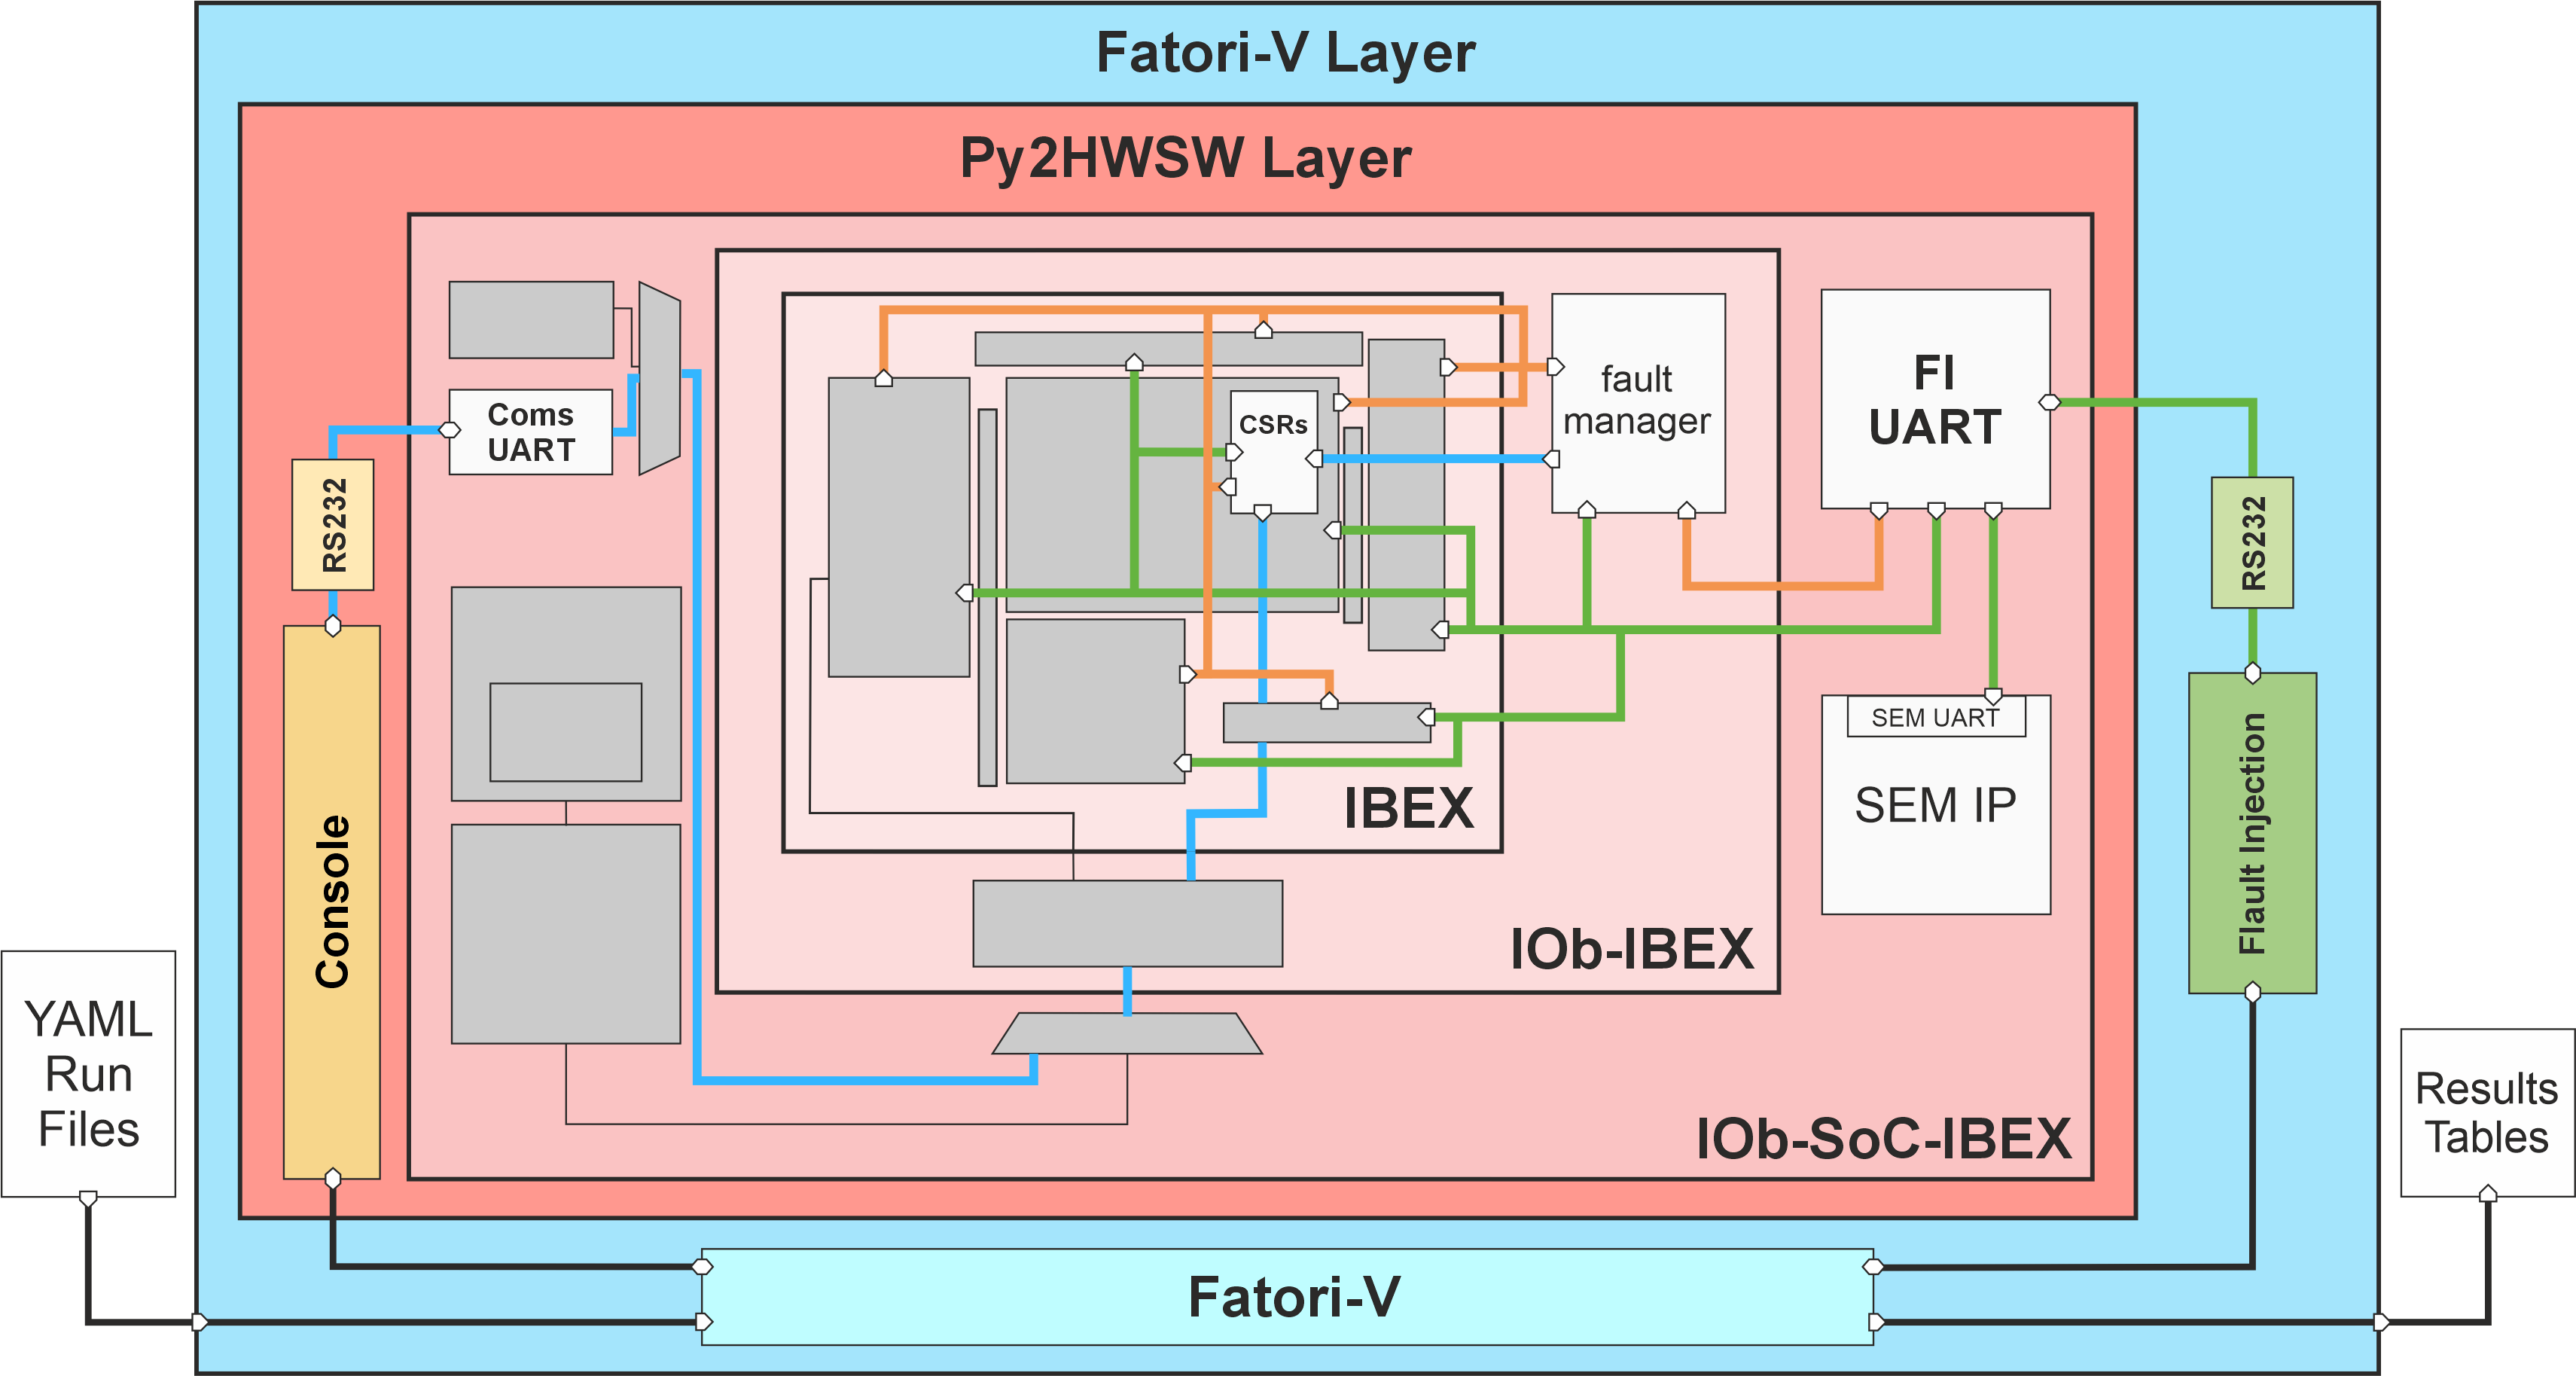
\includegraphics[width=0.9\linewidth]{Images/chap9_exp_setup.png}
  \caption{Fatori-V system used in the experimental setup.}
  \label{fig:chap9_exp_setup}
\end{figure}

\Cref{fig:chap9_exp_setup} shows the system used in the experiments. The \texttt{fatori-v.py} script runs all \texttt{.yaml} tests. Each test synthesizes and implements the FPGA hardware, programs the FPGA, configures the \ac{FI}, and waits for the firmware to finish execution. Next, the text file produced by the firmware, containing the measured results, is analyzed to generate the result tables.

%orange
All \acp{FTM} implemented in this work report their error signals to the central \texttt{fault manager} (orange paths in \cref{fig:chap9_exp_setup}). The fault manager writes the error data to the implemented Ibex \acp{CSR}.

%blue
The firmware reads the \acp{CSR} and sends the metrics to the user desktop console (blue path in \cref{fig:chap9_exp_setup}). The \ac{Fatori-V} platform parses the results and consolidates them into the tables used in the analyses presented below.

%green
During execution, faults are injected (green paths in \cref{fig:chap9_exp_setup}) using the \ac{FI} \ac{UART}, and decoded either as "R" commands (register injections), or \ac{SEM} commands (configuration-memory injections).


%####################################################################
\section{Fatori-V Validation} 
\label{chap9:fatori_validation} 

Before evaluating the \acp{FTM}, a set of experiments was performed to validate \ac{Fatori-V} itself, focusing on whether faults are injected in the intended area and whether the implemented time distributions match their configuration.

The area precision was evaluated through the Pblock Model. For each pblock target, the estimated target size was compared with the real required size reported afterwards by Vivado, using the normalized absolute difference between the two values with \(A = 100*|S_{\mathrm{real}} - S_{\mathrm{est}}|/S_{\mathrm{est}}\). Targets with configurable parameters (such as the \ac{ALU}, the Controller, and others) were evaluated in the baseline configuration and two increasingly complex extra configurations. Targets without configurable parameters (such as the Writeback Stage, the Prefetch Buffer or the Branch Predictor) were evaluated once. The Pblock Model accuracy results are shown in \cref{fig:chap9-pblock-model-accuracy}.

\begin{figure}[h]
    \centering
    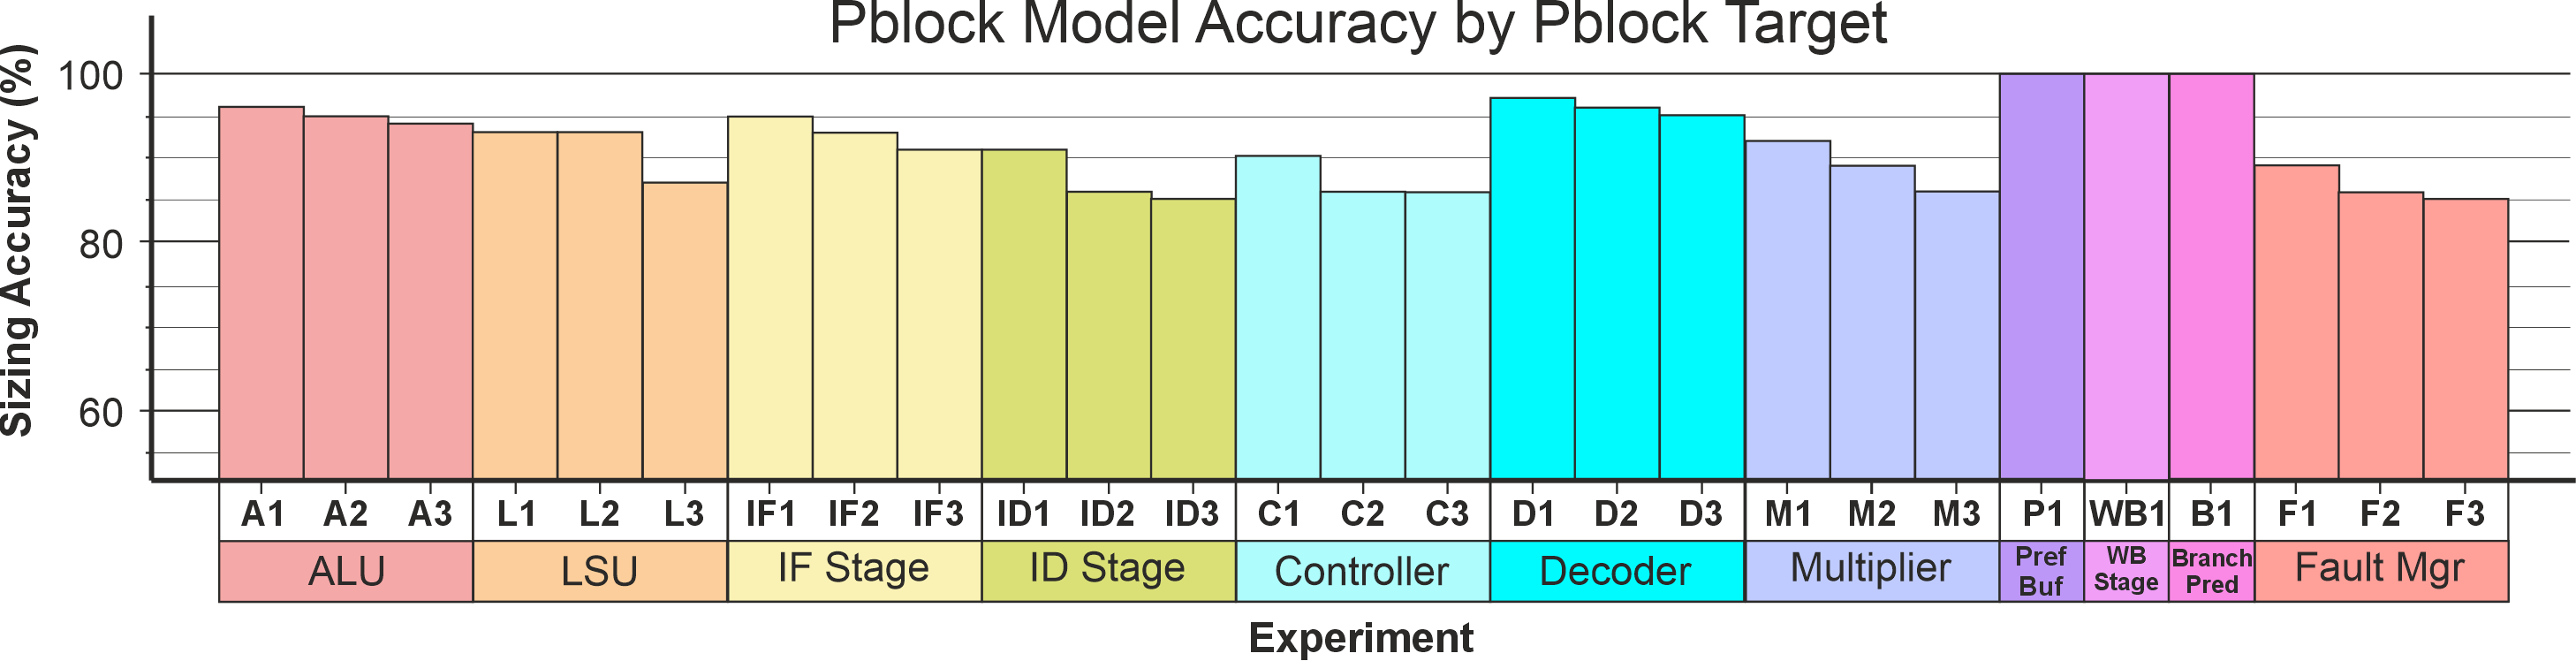
\includegraphics[width=0.9\textwidth]{Images/chap9_pblock_model_accuracy.png}
    \caption{Pblock Model accuracy across the evaluated pblock targets.}
    \label{fig:chap9-pblock-model-accuracy}
\end{figure} 

The Pblock Model reached 100\% accuracy in non-configurable targets, such as the Branch Predictor or the Prefetch Buffer, 85\% in the most complex configurations of parameterizable targets, such as the ID Stage and the \ac{LSU}, and 91.63\% on average. The lower scores occur in targets that allow the most configuration (features with different implementations, replication factors, and others).

The time profiles were evaluated by running timestamped \ac{FI} campaigns for each implemented profile. Each campaign was configured to produce approximately 12000 injections. The measured timestamps were then used to reconstruct the observed behaviour and compare it with the ideal profile generated from the same configuration. The Uniform, Poisson, and \ac{MMPP2} profiles are evaluated as inter-injection period distributions, while Ramp and Microburst profiles are evaluated as timestamp-derived local rate profiles.


\begin{figure}[h]
    \centering
    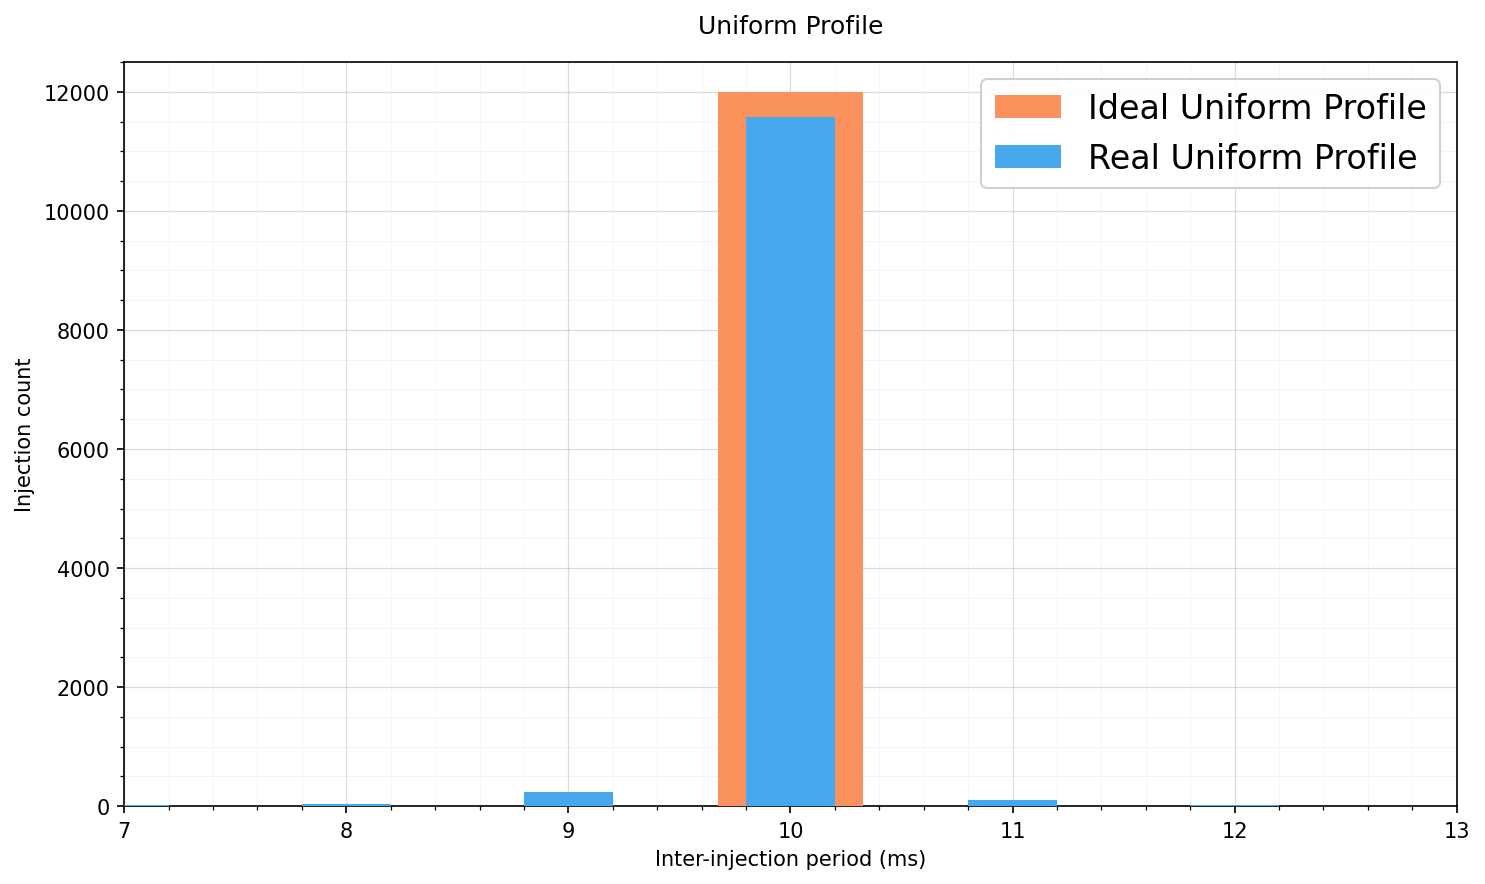
\includegraphics[width=0.7\linewidth]{Images/uniform_profile_overlay.png}
    \caption{Uniform profile.}
    \label{fig:chap9-uniform-profile}
\end{figure} 
% \begin{figure}[h]
%     \centering
%     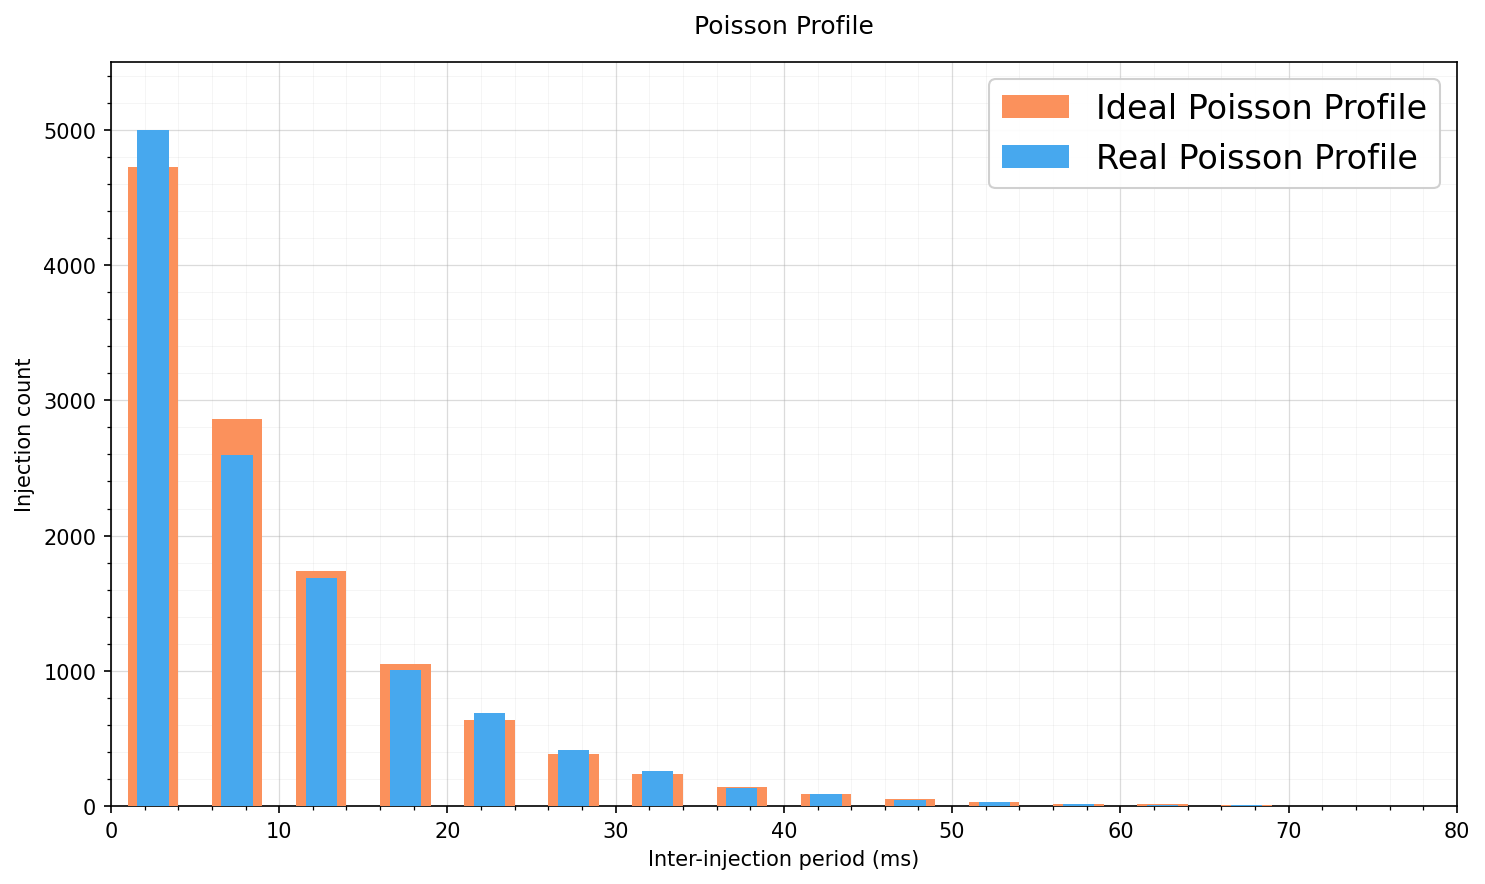
\includegraphics[width=0.8\linewidth]{Images/poisson_profile_overlay.png}
%     \caption{Poisson profile.}
%     \label{fig:chap9-poisson-profile}
% \end{figure} 
% \begin{figure}[h]
%     \centering
%     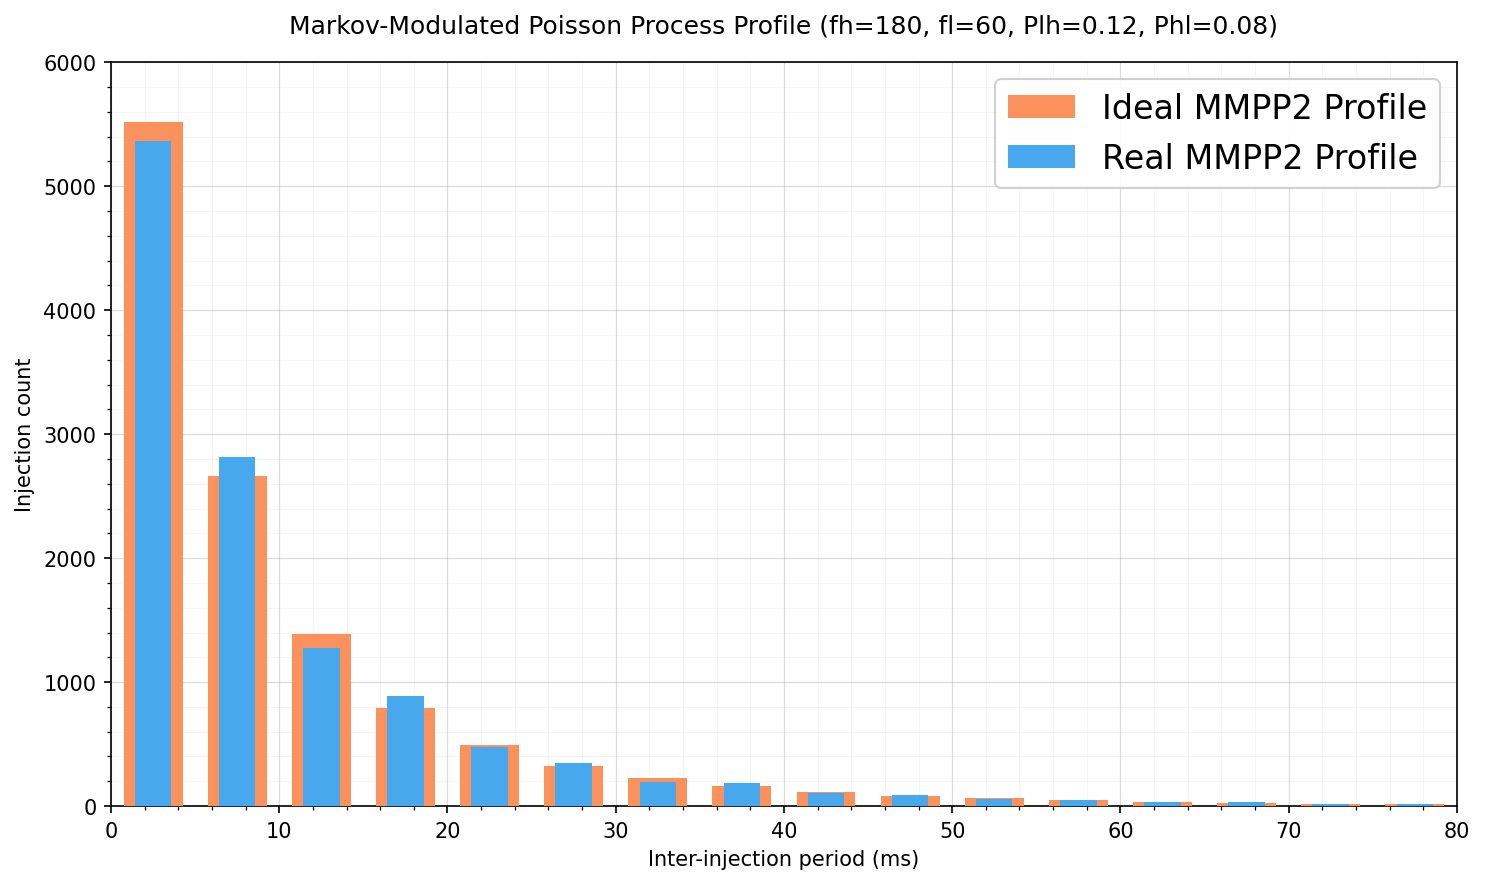
\includegraphics[width=0.8\linewidth]{Images/mmpp2_profile_overlay.png}
%     \caption{\ac{MMPP2} profile.}
%     \label{fig:chap9-mmpp2-profile}
% \end{figure}
% \begin{figure}[h]
%     \centering
%     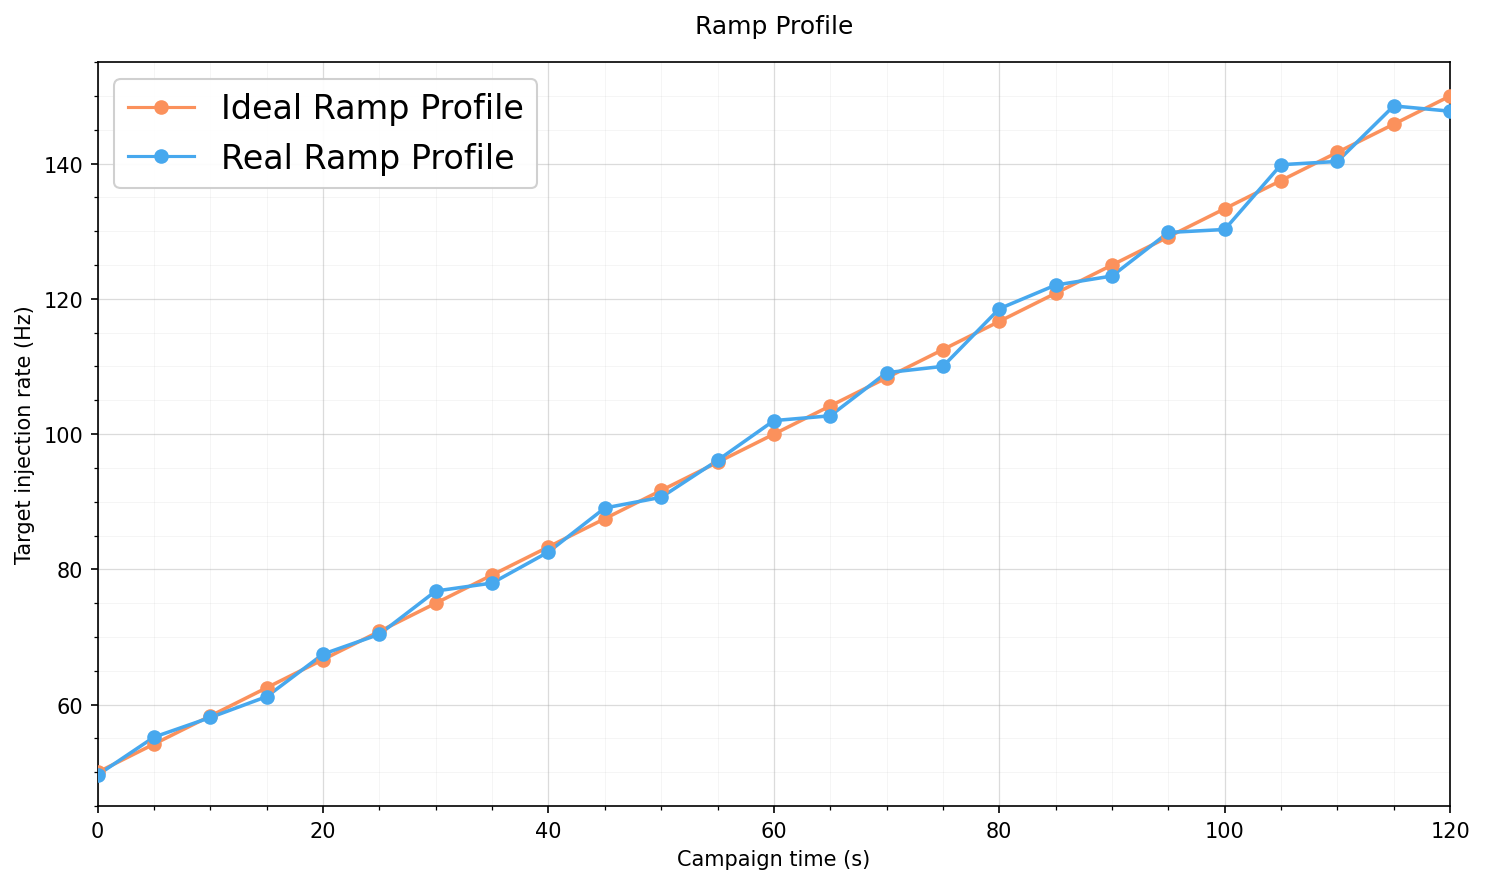
\includegraphics[width=0.8\linewidth]{Images/ramp_profile_line.png}
%     \caption{Ramp profile.}
%     \label{fig:chap9-ramp-profile}
% \end{figure} 
% \begin{figure}[h]
%     \centering
%     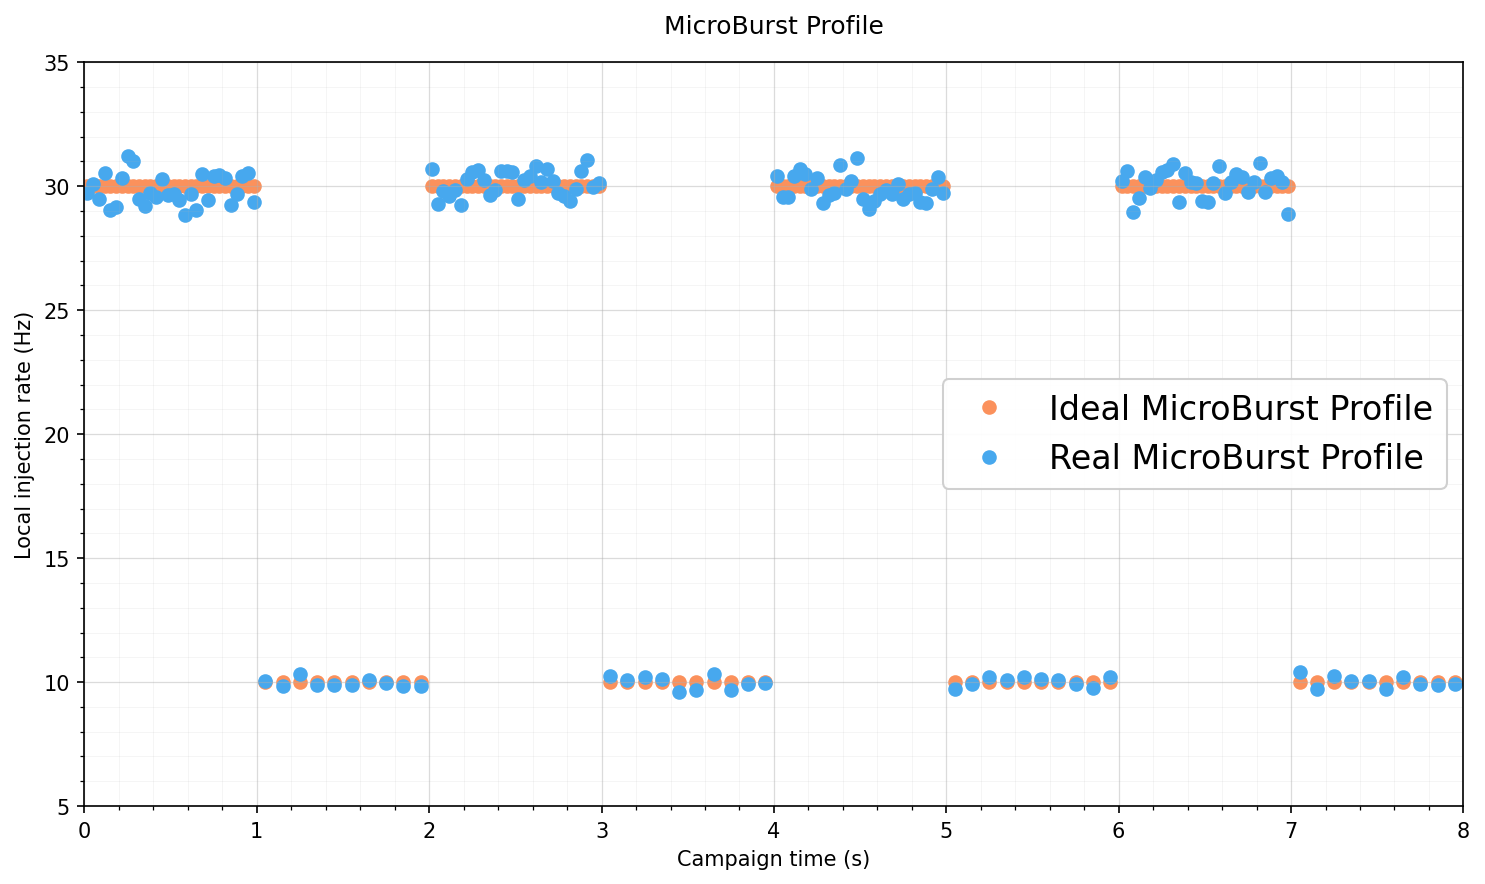
\includegraphics[width=0.8\linewidth]{Images/microburst_profile_unconnected.png}
%     \caption{Microburst profile.}
%     \label{fig:chap9-microburst-profile}
% \end{figure}


\begin{figure}[h]
    \centering
    \begin{subfigure}{0.48\textwidth}
        \centering
        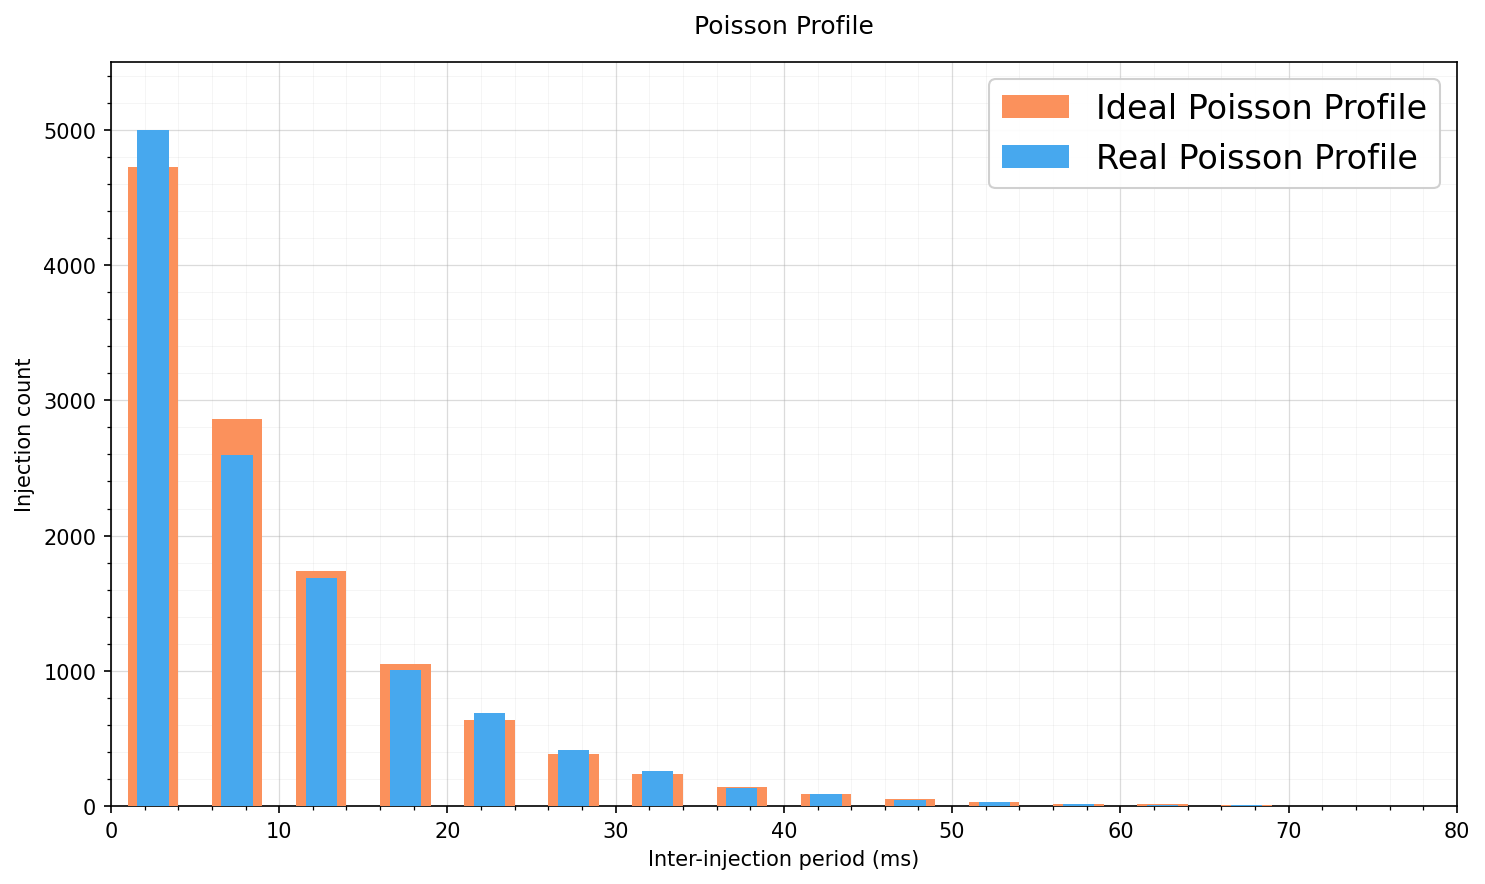
\includegraphics[width=\linewidth]{Images/poisson_profile_overlay.png}
        \caption{Poisson profile.}
        \label{fig:chap9-poisson-profile}
    \end{subfigure}
    \hfill
    \begin{subfigure}{0.48\textwidth}
        \centering
        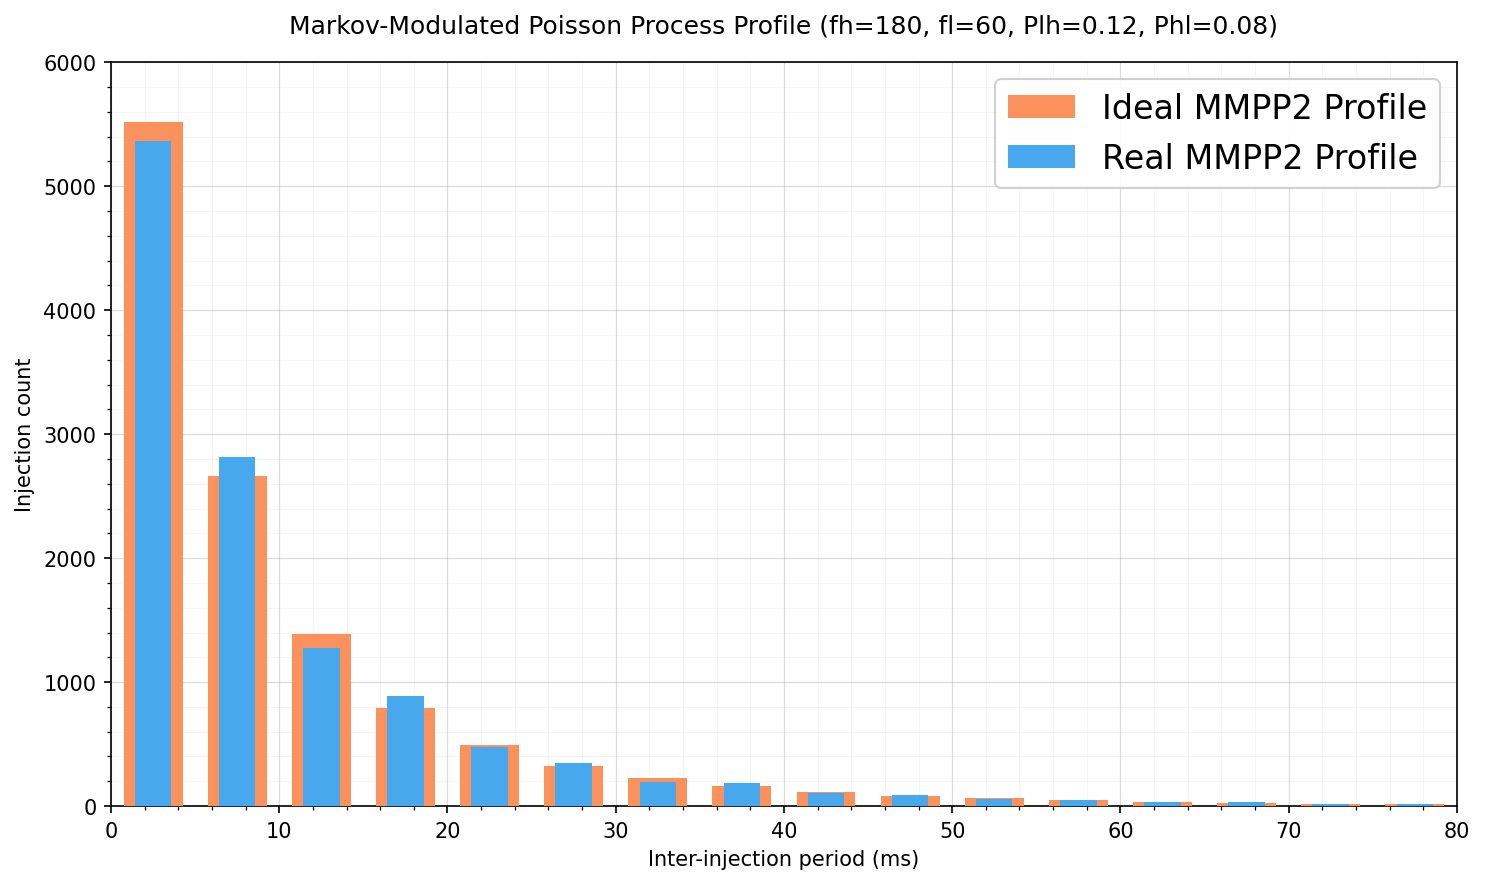
\includegraphics[width=\linewidth]{Images/mmpp2_profile_overlay.png}
        \caption{\ac{MMPP2} profile.}
        \label{fig:chap9-mmpp2-profile}
    \end{subfigure}
    \caption{Poisson and \ac{MMPP2} time profiles validation.}
    \label{fig:chap9-poisson-profiles}
\end{figure}

\begin{figure}[h]
    \centering
    \begin{subfigure}{0.48\textwidth}
        \centering
        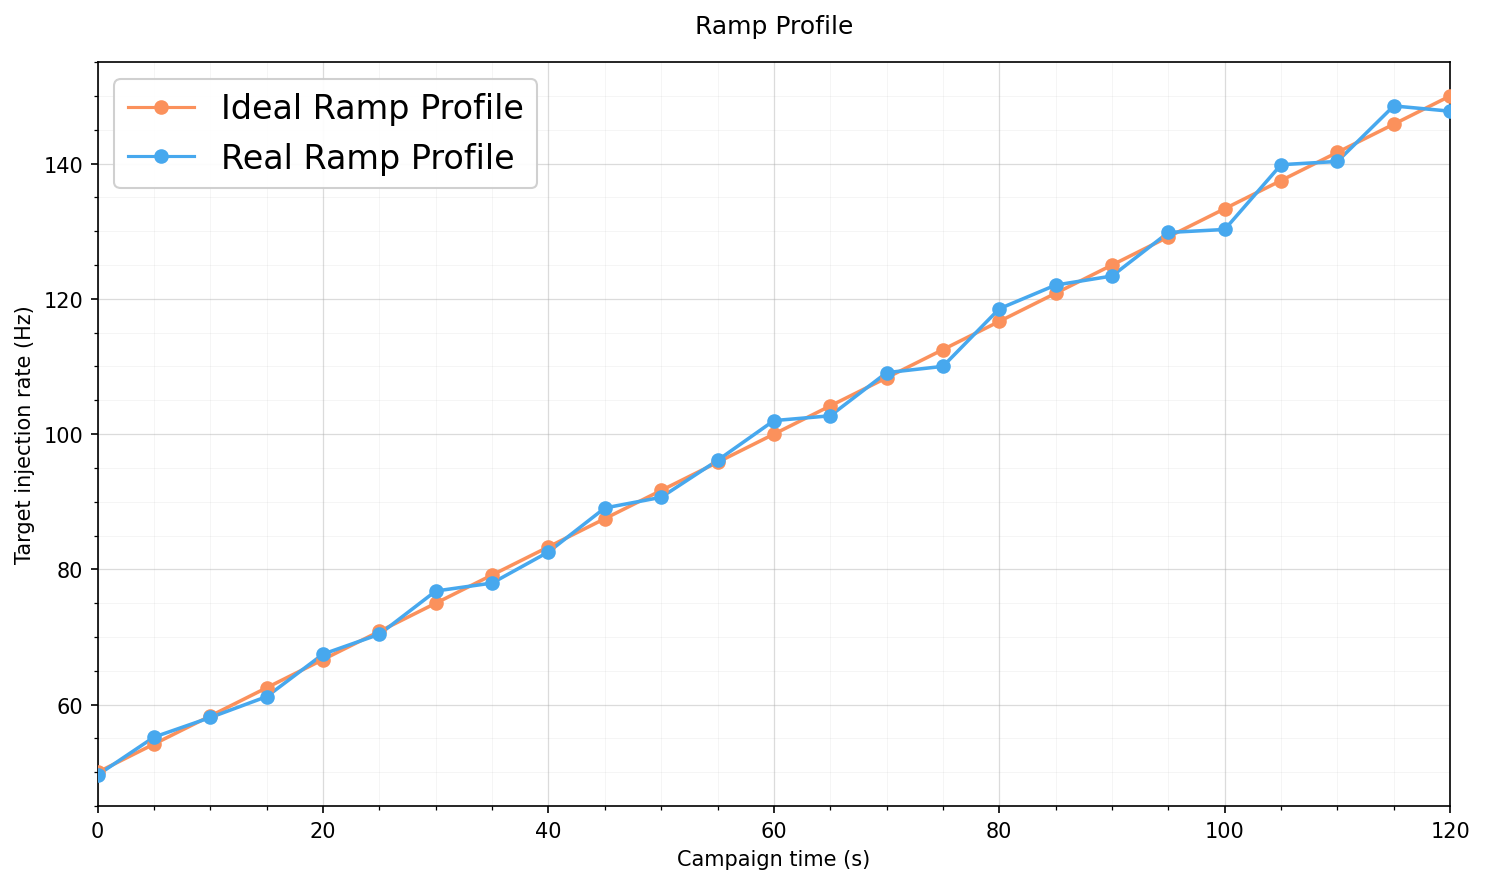
\includegraphics[width=\linewidth]{Images/ramp_profile_line.png}
        \caption{Ramp profile.}
        \label{fig:chap9-ramp-profile}
    \end{subfigure}
    \hfill
    \begin{subfigure}{0.48\textwidth}
        \centering
        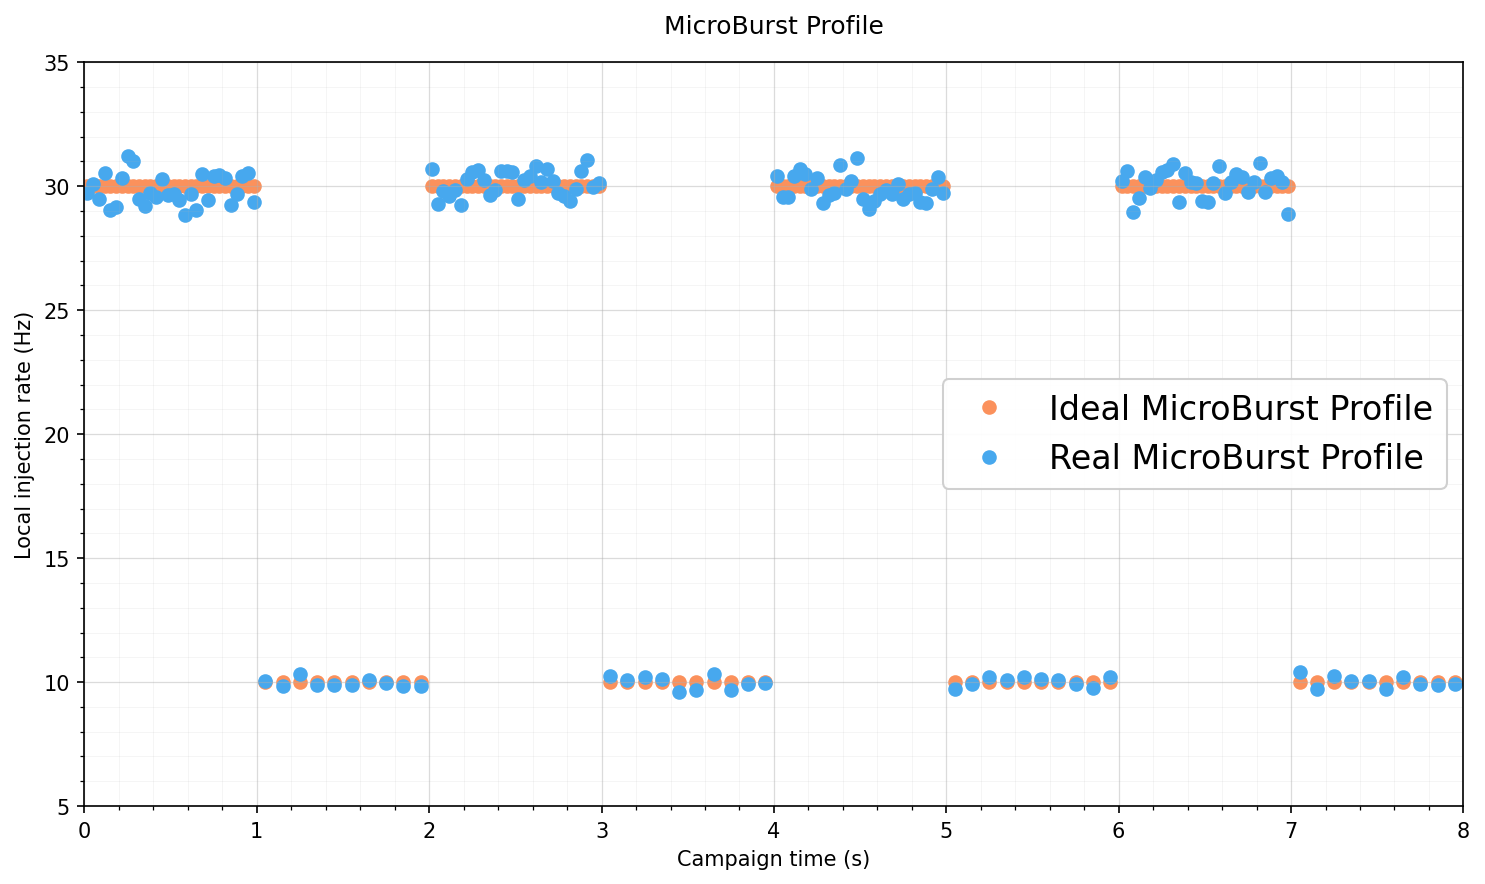
\includegraphics[width=\linewidth]{Images/microburst_profile_unconnected.png}
        \caption{Microburst profile.}
        \label{fig:chap9-microburst-profile}
    \end{subfigure}
    \caption{Ramp and Microburst time profiles validation.}
    \label{fig:chap9-ramp-microburst-profiles}
\end{figure}

The Uniform and Poisson profiles in \cref{fig:chap9-uniform-profile,fig:chap9-poisson-profile} were configured with a 100 Hz mean rate, corresponding to an expected 10 ms mean period, and the measured distributions concentrate around that value. The \ac{MMPP2} profile combines a 60 Hz low-rate state and a 180 Hz high-rate state, with transition probabilities of 0.12 from low to high and 0.08 from high to low. These probabilities give stationary proportions of 0.40 and 0.60, resulting in an expected mean period of \(0.40 \cdot 1000/60 + 0.60 \cdot 1000/180 = 10\ \mathrm{ms}\), which is confirmed by \cref{fig:chap9-mmpp2-profile}. The Ramp and Microburst results in \cref{fig:chap9-ramp-profile,fig:chap9-microburst-profile} confirm their intended behaviour.

\Cref{tab:chap9-time-profile-accuracy} shows the accuracy of each measured profile against the ideal profile generated with the same configuration, using the accuracy equation defined above.

\begin{table}[h]
\centering
\scriptsize
\setlength{\tabcolsep}{3pt}
\renewcommand{\arraystretch}{1.15}
\begin{tabularx}{0.8\textwidth}{|X|X|}
\hline
Time profile &
Profile match \\
\hline
\hline
Uniform &
96.50\% \\
\hline
Poisson &
96.80\% \\
\hline
\ac{MMPP2} &
97.24\% \\
\hline
Ramp &
98.64\% \\
\hline
Microburst &
98.40\% \\
\hline
\end{tabularx}
\caption{Time profile validation scores obtained from the timestamp logs.}
\label{tab:chap9-time-profile-accuracy}
\end{table}





% #############################################################################
\section{Comparison of Fault Tolerance Mechanisms}
\label{chap9:general-ftm-testing}


This section performs the comparison mentioned in \cref{chap1:motivation} by evaluating 11 \acp{FTM}, an Ibex baseline, the native SecureIbex \ac{FTM} set, and a system with all implemented \acp{FTM} enabled. The native Ibex \acp{FTM} considered in this comparison are Lockstep, Dummy Instructions, Data Independent Timing, Hardened \ac{PC}, PMP, RegFile \ac{ECC}, RegFile RADDR glitch checks, \ac{RF} WE glitch checks, Secure Guards, and Shadow \acp{CSR}. The two \acp{FTM} implemented for \ac{Fatori-V} are Register Redundancy (Register M-of-N), and Logic Redundancy (Logic M-of-N). Register M-of-N was enabled for all 197 wrapped registers, with $N=3$, $M=2$, with the correction feature enabled. Logic M-of-N was enabled for all five supported logic targets listed in \cref{chap6:mon} (\ac{ALU}, \ac{LSU}, Controller, Decoder, and IF Stage) with $N=3$ and $M=2$. 

The Baseline contains no \acp{FTM}, but keeps the Fault Manager Redundancyitoring hardware enabled because these are required to retrieve \ac{FT} data. The Baseline uses Branch Predictor and Branch Target \ac{ALU}, and enables the M, C, and B \ac{ISA} extensions. The multiplier is the native Ibex Single Cycle multiplier, and the bit manipulation unit is the native Ibex Balanced implementation.

The comparison uses one configuration per \ac{FTM}, with only that \ac{FTM} enabled. It also includes the Baseline, SecureIbex, which enables only Ibex's native \acp{FTM}, and one configuration with all \acp{FTM} enabled. For each configuration, \ac{Fatori-V} executes the same set of \ac{FI} experiments by varying the injection rate, the register/configuration ratio, and the injection scope, resulting in 588 experiments.

The \ac{FI} campaigns use two injection scopes, the full device and the selected Pblock targets. All injections use the Poisson time profile, a fixed duration of 120 s, and injection rates of 1 Hz, 10 Hz, 50 Hz, 100 Hz, 500 Hz, 1000 Hz, and 5000 Hz. The register/configuration ratio controls the distribution of injections between registers and configuration memory. A ratio of 0 injects only configuration faults, a ratio of 1 injects only register faults, and a ratio of 0.0001 combines both fault types. The mixed ratio approximates the proportion between the 197 wrapped registers and the 1837420 \ac{EBD} configuration addresses, since $197/1837420\approx0.0001$. \ac{Fatori-V} uses fixed seeds, the same benchmarks, and the same \ac{FI} configuration across experiments to keep them comparable. The \ac{FI} target pool from the first experiment was reused in the remaining experiments, so that each campaign followed the same injection targets and timing.

The experiments ran the software benchmarks included with \ac{Fatori-V}, which were Fatori Stress with 100000 iterations and all targets enabled, CoreMark with 1000 iterations, and the Embench-IoT benchmarks crc32, cubic, edn, huffbench, matmult\_int, md5sum, minver, nbody, nettle\_aes, and nettle\_sha256. The benchmarks were configured to run until completion. The performance results were measured from CoreMark and Embench-IoT runs and experiment success was measured with Fatori Stress's checksum check.







\subsection{Fault Tolerance}

\Cref{tab:results_wd_all_ratios,tab:results_modules_all_ratios} summarize the results for the whole-device and Pblock-target injection scopes.

The primary method for evaluating \ac{FT} is to identify which \acp{FTM} allow the system to execute correctly under \ac{FI}. In the following tables, a green cell means that the benchmark completed and produced the correct checksum, a yellow cell means that the benchmark completed but produced the wrong checksum, and a red cell means that the system hung, reset, timed out, or did not publish usable metrics.

The percentage values inside the table cells provide a secondary analysis of the \acp{FTM} through Observability, defined as the share of injected faults detected by the enabled \acp{FTM}. They are included to show additional metrics exported by \ac{Fatori-V} and to expand the analysis beyond pass, fail, and crash.


\providecommand{\ftpass}{\cellcolor{green!30}Pass}
\providecommand{\ftfail}{\cellcolor{yellow!50}Fail}
\providecommand{\ftbroke}{\cellcolor{red!20}Crash}
\providecommand{\obspass}[1]{\cellcolor{green!30}#1}
\providecommand{\obsfail}[1]{\cellcolor{yellow!50}#1}


\begin{table}[h]
\centering
\scriptsize
\setlength{\tabcolsep}{2.2pt}
\renewcommand{\arraystretch}{1.15}
\begin{tabularx}{\textwidth}{|c|p{0.15\textwidth}|X|c|c|c|c|c|c|c|}
\hline
Ratio &
\ac{FTM} Subset &
Members &
1 Hz &
10 Hz &
50 Hz &
100 Hz &
500 Hz &
1000 Hz &
5000 Hz \\
\hline
\hline
\multirow{2}{*}{1} &
Native/no Register Redundancy \acp{FTM} &
Baseline, Lockstep, Dummy Instructions, DIT, Hardened \ac{PC}, PMP, RegFile \ac{ECC}, RegFile Glitches, Secure Guards, Shadow \acp{CSR}, SecureIbex, Logic Redundancy &
\ftbroke &
\ftbroke &
\ftbroke &
\ftbroke &
\ftbroke &
\ftbroke &
\ftbroke\\
\cline{2-10}
&
Experiments with Register Redundancy &
Register Redundancy, All \acp{FTM} &
\obspass{26.6667\%} &
\obspass{26.5000\%} &
\obspass{26.4667\%} &
\obspass{26.4583\%} &
\obspass{26.4600\%} &
\obspass{26.4600\%} &
\obspass{26.4600\%}\\
\hline
\hline
\multirow{2}{*}{0} &
Native/no Logic Redundancy \acp{FTM} &
Baseline, Lockstep, Dummy Instructions, DIT, Hardened \ac{PC}, PMP, RegFile \ac{ECC}, RegFile Glitches, Secure Guards, Shadow \acp{CSR}, SecureIbex, Register Redundancy &
\obspass{0.0000\%} &
\obspass{0.0000\%} &
\obspass{0.0000\%} &
\obspass{0.0000\%} &
\obsfail{0.0000\%} &
\ftbroke &
\ftbroke\\
\cline{2-10}
&
Experiments with Logic Redundancy &
Logic Redundancy, All \acp{FTM} &
\obspass{0.0000\%} &
\obspass{0.0833\%} &
\obspass{0.0667\%} &
\obspass{0.0500\%} &
\obspass{0.0150\%} &
\obsfail{0.0075\%} &
\ftbroke\\
\hline
\hline
\multirow{4}{*}{0.0001} &
Native &
Baseline, Lockstep, Dummy Instructions, DIT, Hardened \ac{PC}, PMP, RegFile \ac{ECC}, RegFile Glitches, Secure Guards, Shadow \acp{CSR}, SecureIbex &
\ftbroke &
\ftbroke &
\ftbroke &
\ftbroke &
\ftbroke &
\ftbroke &
\ftbroke\\
\cline{2-10}
&
Experiments with just Logic Redundancy &
Logic Redundancy &
\ftbroke &
\ftbroke &
\ftbroke &
\ftbroke &
\ftbroke &
\ftbroke &
\ftbroke\\
\cline{2-10}
&
Experiments with just Register Redundancy &
Register Redundancy &
\obspass{0.8333\%} &
\obspass{0.0833\%} &
\obspass{0.0167\%} &
\obspass{0.0083\%} &
\obsfail{0.0033\%} &
\ftbroke &
\ftbroke\\
\cline{2-10}
&
Experiments with both Redundancy \acp{FTM} &
All \acp{FTM} &
\obspass{0.8333\%} &
\obspass{0.1667\%} &
\obspass{0.0833\%} &
\obspass{0.0583\%} &
\obspass{0.0183\%} &
\obsfail{0.0100\%} &
\ftbroke\\
\hline
\end{tabularx}
\caption{Whole Device injection scope \ac{FTM} comparison for the three register/configuration ratios.}
\label{tab:results_wd_all_ratios}
\end{table}


\Cref{tab:results_wd_all_ratios} shows that every system without Register Redundancy crashes when register faults are injected. This shows that register faults have stronger impact than configuration memory faults in the studied system. With Register Redundancy, the system passes every register-only rate, validating the implementation for the tested register faults.

Logic Redundancy also improves \ac{FT}. In the ratio 0 experiments, it keeps the benchmark passing for one additional injection rate compared with the configurations without Logic Redundancy. The Observability values for the same ratio show that detection remains low, which is expected because only the replicated logic targets can detect configuration memory faults. This also suggests that many whole-device configuration injections land outside the exercised or protected logic.

In mixed injection experiments, as in any experiment with register injections, Register Redundancy is required. With it, the results become closer to ratio 0 because configuration memory injections dominate the \ac{FI} campaigns.

The native Ibex \acp{FTM} show the poorest results. They do not protect the system against the tested \acp{SEU}, which is consistent with \cref{chap5:ibex_ft}, where most native mechanisms are described as side-channel hardening or specific integrity checks rather than correction mechanisms for register and configuration memory faults.

The whole-device results show the need for a more focused injection scope. The system passes several ratio 0 rates even without Logic Redundancy, and Observability remains low because many configuration memory injections are not detected. To concentrate faults in relevant logic, the same experiments were repeated with the injection scope limited to the Pblock targets described in \cref{chap7:pblock}. This scope depends on the Pblock Model evaluated in \cref{chap9:fatori_validation}, because the \ac{FI} tool uses the generated Pblock regions to select the configuration addresses for each target module. \Cref{tab:results_modules_all_ratios} summarizes the Pblock injection scope results.


\begin{table}[h]
\centering
\scriptsize
\setlength{\tabcolsep}{2.2pt}
\renewcommand{\arraystretch}{1.15}
\begin{tabularx}{\textwidth}{|c|p{0.15\textwidth}|X|c|c|c|c|c|c|c|}
\hline
Ratio &
\ac{FTM} Subset &
Members &
1 Hz &
10 Hz &
50 Hz &
100 Hz &
500 Hz &
1000 Hz &
5000 Hz \\
\hline
\hline
\multirow{2}{*}{1} &
Native/no Register Redundancy \acp{FTM} &
Baseline, Lockstep, Dummy Instructions, DIT, Hardened \ac{PC}, PMP, RegFile \ac{ECC}, RegFile Glitches, Secure Guards, Shadow \acp{CSR}, SecureIbex, Logic Redundancy &
\ftbroke &
\ftbroke &
\ftbroke &
\ftbroke &
\ftbroke &
\ftbroke &
\ftbroke\\
\cline{2-10}
&
Experiments with Register Redundancy &
Register Redundancy, All \acp{FTM} &
\obspass{26.6667\%} &
\obspass{26.5000\%} &
\obspass{26.4667\%} &
\obspass{26.4583\%} &
\obspass{26.4600\%} &
\obspass{26.4600\%} &
\obspass{26.4600\%}\\
\hline
\hline
\multirow{2}{*}{0} &
Native/no Logic Redundancy \acp{FTM} &
Baseline, Lockstep, Dummy Instructions, DIT, Hardened \ac{PC}, PMP, RegFile \ac{ECC}, RegFile Glitches, Secure Guards, Shadow \acp{CSR}, SecureIbex, Register Redundancy &
\obspass{0.0000\%} &
\obspass{0.0000\%} &
\obsfail{0.0000\%} &
\obsfail{0.0000\%} &
\ftbroke &
\ftbroke &
\ftbroke\\
\cline{2-10}
&
Experiments with Logic Redundancy &
Logic Redundancy, All \acp{FTM} &
\obspass{0.0000\%} &
\obspass{0.1667\%} &
\obspass{0.1000\%} &
\obspass{0.0583\%} &
\obsfail{0.0150\%} &
\ftbroke &
\ftbroke\\
\hline
\hline
\multirow{4}{*}{0.0001} &
Native &
Baseline, Lockstep, Dummy Instructions, DIT, Hardened \ac{PC}, PMP, RegFile \ac{ECC}, RegFile Glitches, Secure Guards, Shadow \acp{CSR}, SecureIbex &
\ftbroke &
\ftbroke &
\ftbroke &
\ftbroke &
\ftbroke &
\ftbroke &
\ftbroke\\
\cline{2-10}
&
Experiments with just Logic Redundancy &
Logic Redundancy &
\ftbroke &
\ftbroke &
\ftbroke &
\ftbroke &
\ftbroke &
\ftbroke &
\ftbroke\\
\cline{2-10}
&
Experiments with just Register Redundancy &
Register Redundancy &
\obspass{0.8333\%} &
\obspass{0.0833\%} &
\obsfail{0.0167\%} &
\obsfail{0.0083\%} &
\ftbroke &
\ftbroke &
\ftbroke\\
\cline{2-10}
&
Experiments with both Redundancy \acp{FTM} &
All \acp{FTM} &
\obspass{0.8333\%} &
\obspass{0.2500\%} &
\obspass{0.1167\%} &
\obspass{0.0667\%} &
\obsfail{0.0183\%} &
\ftbroke &
\ftbroke\\
\hline
\end{tabularx}
\caption{Pblock targets injection scope \ac{FTM} comparison for the three register/configuration ratios.}
\label{tab:results_modules_all_ratios}
\end{table}

Comparing \cref{tab:results_wd_all_ratios,tab:results_modules_all_ratios} shows that the Pblock-target scope makes configuration memory faults fail the system earlier. Without Logic Redundancy, the first failure rate drops by 10 times, from 500 Hz to 50 Hz. With Logic Redundancy, it drops by 2 times, from 1000 Hz to 500 Hz. The smaller drop with Logic Redundancy shows that it protects the system against logic corruption.

For experiments with ratio 1 and Register Redundancy enabled, the system passes every tested rate, but Observability remains close to 26.5\%, instead of 100\%. This suggests a limitation in the aggregation and counting path, rather than in the correction mechanism, caused by the merge of detection signals before being counted.

For experiments with ratio 0, Observability remains low and decreases as the injection rate increases. This shows two limits of the current Logic Redundancy implementation. First, only five logic targets can detect configuration memory faults. Second, detected faults are not repaired, so detections are capped and additional injections do not lead to a proportional increase in detections.

% A third analysis uses the \ac{EBD} counts exported by the \ac{Fatori-V}, which report how many \ac{EBD} bits belong to the complete \ac{SoC} and to each Pblock. The goal was to estimate how much configuration memory corruption the system tolerates in each scope. The estimated corruption is computed by dividing the number of configuration injections by the number of \ac{EBD} bits in the selected scope. \Cref{tab:chap9-ebd-scopes} reports this estimate for the ratio 0 campaigns, comparing both injection scopes with and without Logic M-of-N.

% \begin{table}[h]
% \centering
% \scriptsize
% \setlength{\tabcolsep}{1.6pt}
% \renewcommand{\arraystretch}{1.15}
% \resizebox{\textwidth}{!}{%
% \begin{tabular}{|p{0.14\textwidth}|p{0.13\textwidth}|c|c|r|r|r|c|r|c|c|}
% \hline
% Injection scope &
% Configuration &
% Rate &
% Status &
% Cfg. inj. &
% Scope \ac{EBD} &
% \ac{SoC} \ac{EBD} &
% Logic M-of-N \ac{EBD} / Scope &
% Est. Logic M-of-N inj. &
% \ac{SoC} corr. &
% Scope corr. \\
% \hline
% \hline
% Whole \ac{SoC} &
% Without Logic M-of-N &
% 1 Hz &
% \ftpass &
% 120 &
% 1837420 &
% 1837420 &
% -- &
% -- &
% 0.0065\% &
% 0.0065\% \\
% \cline{3-11}
% &
% &
% 10 Hz &
% \ftpass &
% 1200 &
% 1837420 &
% 1837420 &
% -- &
% -- &
% 0.0653\% &
% 0.0653\% \\
% \cline{3-11}
% &
% &
% 50 Hz &
% \ftpass &
% 6000 &
% 1837420 &
% 1837420 &
% -- &
% -- &
% 0.3265\% &
% 0.3265\% \\
% \cline{3-11}
% &
% &
% 100 Hz &
% \ftpass &
% 12000 &
% 1837420 &
% 1837420 &
% -- &
% -- &
% 0.6531\% &
% 0.6531\% \\
% \cline{3-11}
% &
% &
% 500 Hz &
% \ftfail &
% 60000 &
% 1837420 &
% 1837420 &
% -- &
% -- &
% 3.2654\% &
% 3.2654\% \\
% \cline{3-11}
% &
% &
% 1000 Hz &
% \ftbroke &
% 120000 &
% 1837420 &
% 1837420 &
% -- &
% -- &
% 6.5309\% &
% 6.5309\% \\
% \cline{3-11}
% &
% &
% 5000 Hz &
% \ftbroke &
% 600000 &
% 1837420 &
% 1837420 &
% -- &
% -- &
% 32.6545\% &
% 32.6545\% \\
% \hline
% Whole \ac{SoC} &
% With Logic M-of-N &
% 1 Hz &
% \ftpass &
% 120 &
% 2672260 &
% 2672260 &
% 834840 / 31.24\% &
% 37 &
% 0.0045\% &
% 0.0045\% \\
% \cline{3-11}
% &
% &
% 10 Hz &
% \ftpass &
% 1200 &
% 2672260 &
% 2672260 &
% 834840 / 31.24\% &
% 375 &
% 0.0449\% &
% 0.0449\% \\
% \cline{3-11}
% &
% &
% 50 Hz &
% \ftpass &
% 6000 &
% 2672260 &
% 2672260 &
% 834840 / 31.24\% &
% 1874 &
% 0.2245\% &
% 0.2245\% \\
% \cline{3-11}
% &
% &
% 100 Hz &
% \ftpass &
% 12000 &
% 2672260 &
% 2672260 &
% 834840 / 31.24\% &
% 3749 &
% 0.4491\% &
% 0.4491\% \\
% \cline{3-11}
% &
% &
% 500 Hz &
% \ftpass &
% 60000 &
% 2672260 &
% 2672260 &
% 834840 / 31.24\% &
% 18745 &
% 2.2453\% &
% 2.2453\% \\
% \cline{3-11}
% &
% &
% 1000 Hz &
% \ftfail &
% 120000 &
% 2672260 &
% 2672260 &
% 834840 / 31.24\% &
% 37489 &
% 4.4906\% &
% 4.4906\% \\
% \cline{3-11}
% &
% &
% 5000 Hz &
% \ftbroke &
% 600000 &
% 2672260 &
% 2672260 &
% 834840 / 31.24\% &
% 187446 &
% 22.4529\% &
% 22.4529\% \\
% \hline
% Pblock targets &
% Without Logic M-of-N &
% 1 Hz &
% \ftpass &
% 120 &
% 508940 &
% 1837420 &
% -- &
% -- &
% 0.0065\% &
% 0.0236\% \\
% \cline{3-11}
% &
% &
% 10 Hz &
% \ftpass &
% 1200 &
% 508940 &
% 1837420 &
% -- &
% -- &
% 0.0653\% &
% 0.2358\% \\
% \cline{3-11}
% &
% &
% 50 Hz &
% \ftfail &
% 6000 &
% 508940 &
% 1837420 &
% -- &
% -- &
% 0.3265\% &
% 1.1789\% \\
% \cline{3-11}
% &
% &
% 100 Hz &
% \ftfail &
% 12000 &
% 508940 &
% 1837420 &
% -- &
% -- &
% 0.6531\% &
% 2.3578\% \\
% \cline{3-11}
% &
% &
% 500 Hz &
% \ftbroke &
% 60000 &
% 508940 &
% 1837420 &
% -- &
% -- &
% 3.2654\% &
% 11.7892\% \\
% \cline{3-11}
% &
% &
% 1000 Hz &
% \ftbroke &
% 120000 &
% 508940 &
% 1837420 &
% -- &
% -- &
% 6.5309\% &
% 23.5784\% \\
% \cline{3-11}
% &
% &
% 5000 Hz &
% \ftbroke &
% 600000 &
% 508940 &
% 1837420 &
% -- &
% -- &
% 32.6545\% &
% 117.8921\% \\
% \hline
% Pblock targets &
% With Logic M-of-N &
% 1 Hz &
% \ftpass &
% 120 &
% 1343780 &
% 2672260 &
% 834840 / 62.13\% &
% 75 &
% 0.0045\% &
% 0.0089\% \\
% \cline{3-11}
% &
% &
% 10 Hz &
% \ftpass &
% 1200 &
% 1343780 &
% 2672260 &
% 834840 / 62.13\% &
% 746 &
% 0.0449\% &
% 0.0893\% \\
% \cline{3-11}
% &
% &
% 50 Hz &
% \ftpass &
% 6000 &
% 1343780 &
% 2672260 &
% 834840 / 62.13\% &
% 3728 &
% 0.2245\% &
% 0.4465\% \\
% \cline{3-11}
% &
% &
% 100 Hz &
% \ftpass &
% 12000 &
% 1343780 &
% 2672260 &
% 834840 / 62.13\% &
% 7455 &
% 0.4491\% &
% 0.8930\% \\
% \cline{3-11}
% &
% &
% 500 Hz &
% \ftfail &
% 60000 &
% 1343780 &
% 2672260 &
% 834840 / 62.13\% &
% 37276 &
% 2.2453\% &
% 4.4650\% \\
% \cline{3-11}
% &
% &
% 1000 Hz &
% \ftbroke &
% 120000 &
% 1343780 &
% 2672260 &
% 834840 / 62.13\% &
% 74551 &
% 4.4906\% &
% 8.9300\% \\
% \cline{3-11}
% &
% &
% 5000 Hz &
% \ftbroke &
% 600000 &
% 1343780 &
% 2672260 &
% 834840 / 62.13\% &
% 372757 &
% 22.4529\% &
% 44.6502\% \\
% \hline
% \end{tabular}%
% }
% \caption{Configuration \ac{EBD} scopes and estimated corruption for all tested injection rates.}
% \label{tab:chap9-ebd-scopes}
% \label{tab:chap9-corruption-estimates}
% \end{table}

% \Cref{tab:chap9-ebd-scopes} suggests that the system fails when the selected scope reaches estimated corruption levels around 1.1789\% to 3.2654\% without Logic M-of-N, and around 4.4650\% to 4.4906\% with Logic M-of-N. The last passing points also move upward, from 0.2358\%--0.6531\% without Logic M-of-N to 0.8930\%--2.2453\% with Logic M-of-N. This supports that Logic M-of-N increases the corruption required before the benchmark starts failing.

% The crash transition is less precise because these values come from the seven injection rates used in the general comparison. Across the two scopes, the system crashes between 2.3578\%--3.2654\% and 6.5309\%--11.7892\% without Logic M-of-N, and between 4.4650\%--4.4906\% and 8.9300\%--22.4529\% with Logic M-of-N. These values estimate corruption inside the selected injection scope, not uniform \ac{SoC}-wide corruption or corruption of one specific target. More injection rates around each transition point would be required to locate the fail and crash thresholds more precisely.



\subsection{Performance and Hardware Resources}

The experiments in \cref{tab:results_wd_all_ratios,tab:results_modules_all_ratios} showed no changes in performance. All runs reported \ac{IPC}=0.28, CoreMark score 44, and Embench-IoT score 0.076. Since \ac{Fatori-V} was not optimized for performance, the constant result suggests that the bottleneck is outside the tested \acp{FTM}, possibly in the \ac{AXI}-to-Ibex bridge described detailed in \cref{chap5:ibex2iob}. \Cref{tab:chap9-general-ftm-perf-hw} focuses on hardware cost and timing.

Native Ibex \acp{FTM} have low or moderate cost, but did not improve the pass, fail, and crash results. Register Redundancy and Logic Redundancy add more hardware, but they are the only individual \acp{FTM} that changed the \ac{FT} results. Register Redundancy protects the system against register faults. Logic Redundancy improves the configuration memory campaigns. SecureIbex combines the native mechanisms and increases cost without improving these results. The All \acp{FTM} configuration has the best \ac{FT} result, but its cost is dominated by mechanisms that did not improve the \ac{FT} results. The best subset would be enabling just Logic and Register Redundancy.

\begin{table}[h]
\centering
\scriptsize
\setlength{\tabcolsep}{3.2pt}
\renewcommand{\arraystretch}{1.15}
\begin{tabularx}{\textwidth}{|p{0.15\textwidth}|X|r|r|c|c|}
\hline
Experiment &
Configuration &
\acp{LUT} &
\acp{FF} &
Power (W) &
Slack (ns) \\
\hline
\hline
\rowcolor{green!25}
Baseline &
Baseline, Fault Manager and Metrics Level HW enabled &
5833 &
3066 &
0.616 &
2.173 \\
\hline
\rowcolor{yellow!10}
Native Ibex &
Simpler than baseline, measurement infrastructure disabled &
4752 &
2304 &
0.590 &
2.518 \\
\hline
\rowcolor{yellow!10}
Lockstep &
Lockstep &
10127 &
5287 &
0.634 &
2.652 \\
\hline
\rowcolor{yellow!10}
Dummy Instructions &
Dummy Instructions &
5915 &
3141 &
0.616 &
3.159 \\
\hline
\rowcolor{yellow!10}
Data Independent Timing &
Data Independent Timing &
5939 &
3066 &
0.619 &
2.282 \\
\hline
\rowcolor{yellow!10}
Hardened \ac{PC} &
Hardened \ac{PC} &
5888 &
3083 &
0.616 &
2.968 \\
\hline
\rowcolor{yellow!10}
PMP &
PMP &
10934 &
3665 &
0.635 &
1.187 \\
\hline
\rowcolor{yellow!10}
Register Redundancy &
Register M-of-N, $N=3$, $M=2$, correction on &
14622 &
6706 &
0.639 &
1.240 \\
\hline
\rowcolor{yellow!10}
Logic Redundancy &
Logic M-of-N, $N=3$, $M=2$, hold off, no correction &
19081 &
7762 &
0.661 &
0.500 \\
\hline
\rowcolor{yellow!10}
RegFile \ac{ECC} &
RegFile \ac{ECC} &
5949 &
3082 &
0.616 &
2.670 \\
\hline
\rowcolor{yellow!10}
RegFile Glitches &
RegFile RADDR/WE glitch checks &
7319 &
4068 &
0.620 &
2.967 \\
\hline
\rowcolor{yellow!10}
Secure Guards &
Secure Guards &
5882 &
3066 &
0.616 &
2.825 \\
\hline
\rowcolor{yellow!10}
Shadow \acp{CSR} &
Shadow \acp{CSR} &
5874 &
3107 &
0.616 &
3.133 \\
\hline
\rowcolor{orange!20}
SecureIbex &
All native \acp{FTM} except both Redundancy \acp{FTM} &
22445 &
9199 &
0.668 &
0.857 \\
\hline
\rowcolor{orange!20}
All \acp{FTM} &
All \acp{FTM} enabled &
107763 &
35661 &
0.779 &
0.020 \\
\hline
\end{tabularx}
\caption{General \ac{FTM} comparison in terms of hardware cost and timing.}
\label{tab:chap9-general-ftm-perf-hw}
\end{table}






% #############################################################################
\section{Register Redundancy}
\label{chap9:register-Redundancy}

\Cref{chap9:general-ftm-testing} already showed that Register M-of-N is required to protect the system from the tested register faults. This section isolates Register M-of-N to evaluate Correction and the replication factor $N$. All experiments use register-only injection campaigns, a whole-device injection scope, and configurations with only the Baseline and Register M-of-N enabled.

\subsection{Fault Tolerance}

\Cref{tab:chap9-regRedundancy-status} displays the Register Redundancy \ac{FT} results. The cell colors have the same meaning as in \cref{chap9:general-ftm-testing}. Green means that the benchmark completed with the correct checksum, yellow means that the benchmark completed with a wrong checksum, and red means that the system crashed, hung, timed out, or did not publish usable metrics.

In addition to the pass, fail, and crash results, the table reports Observability for experiments used to compare how Correction and replication factor affect detection. These values are shown for the $N=3$/$M=2$ injection-rate sweep and for the 10 Hz sweep across different $N$/$M$ values.

\begin{table}[h]
\centering
\scriptsize
\setlength{\tabcolsep}{1.4pt}
\renewcommand{\arraystretch}{1.15}
\begin{tabularx}{\textwidth}{|c|c|c|*{7}{>{\centering\arraybackslash}X|}}
\hline
Correction &
$N$ &
$M$ &
1 Hz &
10 Hz &
50 Hz &
100 Hz &
500 Hz &
1000 Hz &
5000 Hz \\
\hline
\hline
\multirow{6}{*}{on} &
1 &
1 &
\ftbroke &
\ftbroke &
\ftbroke &
\ftbroke &
\ftbroke &
\ftbroke &
\ftbroke \\
\cline{2-10}
&
2 &
2 &
\ftbroke &
\ftbroke &
\ftbroke &
\ftbroke &
\ftbroke &
\ftbroke &
\ftbroke \\
\cline{2-10}
&
3 &
2 &
\obspass{26.6667\%} &
\obspass{26.5000\%} &
\obspass{26.4667\%} &
\obspass{26.4583\%} &
\obspass{26.4600\%} &
\obspass{26.4600\%} &
\obspass{26.4600\%} \\
\cline{2-10}
&
4 &
3 &
\ftpass &
\obspass{26.6250\%} &
\ftpass &
\ftpass &
\ftpass &
\ftpass &
\ftpass \\
\cline{2-10}
&
5 &
3 &
\ftpass &
\obspass{27.0833\%} &
\ftpass &
\ftpass &
\ftpass &
\ftpass &
\ftpass \\
\cline{2-10}
&
7 &
4 &
\ftpass &
\obspass{27.7500\%} &
\ftpass &
\ftpass &
\ftpass &
\ftpass &
\ftpass \\
\hline
\hline
\multirow{6}{*}{off} &
1 &
1 &
\ftbroke &
\ftbroke &
\ftbroke &
\ftbroke &
\ftbroke &
\ftbroke &
\ftbroke \\
\cline{2-10}
&
2 &
2 &
\ftbroke &
\ftbroke &
\ftbroke &
\ftbroke &
\ftbroke &
\ftbroke &
\ftbroke \\
\cline{2-10}
&
3 &
2 &
\obspass{26.7300\%} &
\ftbroke &
\ftbroke &
\ftbroke &
\ftbroke &
\ftbroke &
\ftbroke \\
\cline{2-10}
&
4 &
3 &
\ftpass &
\ftbroke &
\ftbroke &
\ftbroke &
\ftbroke &
\ftbroke &
\ftbroke \\
\cline{2-10}
&
5 &
3 &
\ftpass &
\obsfail{9.4813\%} &
\ftbroke &
\ftbroke &
\ftbroke &
\ftbroke &
\ftbroke \\
\cline{2-10}
&
7 &
4 &
\ftpass &
\obspass{17.4540\%} &
\ftfail &
\ftbroke &
\ftbroke &
\ftbroke &
\ftbroke \\
\hline
\end{tabularx}
\caption{Benchmark results and selected Observability values for the Register M-of-N Correction and $N$ studies.}
\label{tab:chap9-regRedundancy-status}
\end{table}

\Cref{tab:chap9-regRedundancy-status} confirms the result already observed in \cref{chap9:general-ftm-testing}: without an effective register redundancy configuration, register faults crash the system. The new result here is the role of Correction. With $N=3$/$M=2$, Correction enabled passes the full injection-rate sweep, while Correction disabled only passes at 1 Hz.

This difference follows from the Register M-of-N behaviour described in \cref{chap6:mofn_reg}. With Correction disabled, a corrupted replica remains corrupted until the register is overwritten by normal execution. If later injections corrupt enough replicas before that overwrite, the voter can select corrupted data. Correction removes this accumulated state by restoring the corrupted replica after detection.

Increasing $N$ helps the Correction-off case, but does not replace Correction in these experiments. At 10 Hz, $N=7$/$M=4$ without Correction passes, while $N=5$/$M=3$ fails. With Correction enabled, all valid majority configurations pass at 10 Hz, starting at $N=3$/$M=2$. The table therefore supports using Correction before increasing $N$.

The selected Observability values should be read as detection counters, not as a direct measure of correction coverage. With Correction enabled, Observability stays close to 26.5\% for the $N=3$/$M=2$ rate sweep and only increases slightly when $N$ increases at 10 Hz. Since the benchmark still passes every tested rate with Correction enabled, these values are consistent with the aggregation limitation already identified in \cref{chap9:general-ftm-testing}.

\subsection{Performance and Hardware Resources}

The Register M-of-N experiments showed no changes in performance. All configurations reported \ac{IPC}=0.28, CoreMark score 44, and Embench-IoT score 0.076. As in \cref{chap9:general-ftm-testing}, performance is not the limiting factor in this comparison. \Cref{tab:chap9-regRedundancy-cost} focuses on hardware cost and timing.

\begin{table}[h]
\centering
\scriptsize
\setlength{\tabcolsep}{3.0pt}
\renewcommand{\arraystretch}{1.15}
\begin{tabularx}{\textwidth}{|>{\raggedright\arraybackslash}X|c|c|c|r|r|c|c|}
\hline
Configuration &
$N$ &
$M$ &
Correction &
\acp{LUT} &
\acp{FF} &
Power (W) &
Slack (ns) \\
\hline
\hline
\rowcolor{green!25}
Baseline &
1 &
1 &
off &
4752 &
2304 &
0.590 &
2.518 \\
\hline
\rowcolor{yellow!10}
Register M-of-N &
2 &
2 &
on &
9909 &
5899 &
0.611 &
2.135 \\
\hline
\rowcolor{yellow!10}
Register M-of-N &
3 &
2 &
on &
13693 &
7183 &
0.633 &
0.898 \\
\hline
\rowcolor{orange!20}
Register M-of-N &
3 &
2 &
off &
12764 &
5853 &
0.639 &
1.631 \\
\hline
\rowcolor{yellow!10}
Register M-of-N &
4 &
3 &
on &
18567 &
8467 &
0.642 &
0.317 \\
\hline
\rowcolor{yellow!10}
Register M-of-N &
5 &
3 &
on &
24919 &
9868 &
0.675 &
0.151 \\
\hline
\rowcolor{yellow!10}
Register M-of-N &
7 &
4 &
on &
35946 &
12261 &
0.706 &
0.047 \\
\hline
\rowcolor{orange!20}
Register M-of-N &
7 &
4 &
off &
32705 &
9547 &
0.712 &
0.780 \\
\hline
\end{tabularx}
\caption{Register M-of-N hardware cost and timing across the evaluated configurations.}
\label{tab:chap9-regRedundancy-cost}
\end{table}

\Cref{tab:chap9-regRedundancy-cost} shows that the cost grows with $N$, while slack decreases for the Correction-on configurations. At $N=3$/$M=2$, enabling Correction adds 929 \acp{LUT} and 1330 \acp{FF} compared with the same configuration without Correction, but changes the \ac{FT} result from one passing rate to the full injection-rate sweep. The $N=7$/$M=4$ configuration without Correction uses more than twice the \acp{LUT} of $N=3$/$M=2$ with Correction and still fails at 50 Hz. For the tested configurations, $N=3$/$M=2$ with Correction enabled gives the best Register M-of-N result at the lowest hardware cost among the configurations that pass the full rate sweep.











%############################################################################
\section{Logic Redundancy} 
\label{chap9:logic-Redundancy} 

\Cref{chap9:general-ftm-testing} showed that Logic M-of-N was the only tested mechanism that improved execution under configuration memory corruption. This section isolates that mechanism by evaluating the five supported targets (\ac{LSU}, Controller, Decoder, IF Stage, and \ac{ALU}). All experiments use only configuration memory injections, with register/configuration ratio equal to 0.



\subsection{Fault Tolerance}

\Cref{tab:chap9-logicRedundancy-status} reports Benchmark Pass results for two injection scopes. Each experiment enables Logic M-of-N in only one module, shown in the second column. In Whole Device campaigns, injections may affect any part of the \ac{SoC}, while only the listed module is protected. In Target Only campaigns, injections are restricted to the same module that is protected. The Whole Device campaigns use 500 Hz because it was the first failing rate in \cref{tab:results_wd_all_ratios}. The Target Only campaigns use 50 Hz because it was the first failing rate in \cref{tab:results_modules_all_ratios}. The $^{*}$ marks configurations that failed implementation due to timing issues.




\begin{table}[h]
\centering
\scriptsize
\setlength{\tabcolsep}{2.0pt}
\renewcommand{\arraystretch}{1.15}
\begin{tabularx}{\textwidth}{|p{0.16\textwidth}|p{0.13\textwidth}|*{6}{>{\centering\arraybackslash}X|}}
\hline
Injection scope &
Logic M-of-N target &
$N=1$/$M=1$ &
$N=2$/$M=2$ &
$N=3$/$M=2$ &
$N=4$/$M=3$ &
$N=5$/$M=3$ &
$N=7$/$M=4$ \\
\hline
\hline
\multirow{5}{*}{Whole Device, 500 Hz} &
\ac{LSU} &
\ftfail &
\ftfail &
\ftfail &
\ftfail &
\ftfail &
\ftfail \\
\cline{2-8}
&
Controller &
\ftfail &
\ftfail &
\ftfail &
\ftfail &
\ftfail &
\ftfail \\
\cline{2-8}
&
Decoder &
\ftfail &
\ftfail &
\ftfail &
\ftfail &
\ftfail &
\ftfail \\
\cline{2-8}
&
IF Stage &
\ftfail &
\ftfail &
\ftfail &
\ftbroke$^{*}$ &
\ftbroke$^{*}$ &
\ftbroke$^{*}$ \\
\cline{2-8}
&
\ac{ALU} &
\ftfail &
\ftfail &
\ftfail &
\ftfail &
\ftfail &
\ftfail \\
\hline
\hline
\multirow{5}{*}{Target Only, 50 Hz} &
\ac{LSU} &
\ftfail &
\ftfail &
\ftfail &
\ftfail &
\ftpass &
\ftpass \\
\cline{2-8}
&
Controller &
\ftfail &
\ftfail &
\ftpass &
\ftpass &
\ftpass &
\ftpass \\
\cline{2-8}
&
Decoder &
\ftfail &
\ftfail &
\ftpass &
\ftpass &
\ftpass &
\ftpass \\
\cline{2-8}
&
IF Stage &
\ftpass &
\ftpass &
\ftpass &
\ftbroke$^{*}$ &
\ftbroke$^{*}$ &
\ftbroke$^{*}$ \\
\cline{2-8}
&
\ac{ALU} &
\ftfail &
\ftfail &
\ftpass &
\ftpass &
\ftpass &
\ftpass \\
\hline
\end{tabularx}
\caption{Benchmark Pass results for the Logic M-of-N target study.}
\label{tab:chap9-logicRedundancy-status}
\end{table}





The Whole Device rows show that protecting a single Logic M-of-N target is not enough to recover the full \ac{SoC}, because faults can still affect unprotected logic and routing. The Target Only rows isolate each protected module and show the effect of the target and of $N$ more clearly. The \ac{LSU} passes only from $N=5$/$M=3$ onward, which indicates that one tolerated faulty replica is not enough for this target under the selected campaign. The Controller, Decoder, and \ac{ALU} pass from $N=3$/$M=2$ onward, where one faulty replica can be tolerated. The IF Stage passes for the valid configurations, but higher values of $N$ fail implementation due to timing and do not produce valid metrics.

The $N=4$/$M=3$ point does not improve the correction margin over $N=3$/$M=2$, because both tolerate only one faulty replica. The first margin increase appears at $N=5$/$M=3$, which tolerates two corrupted replicas, while $N=7$/$M=4$ tolerates three. The change in Target Only results when $N$ increases also supports the Pblock Model accuracy, because the extra replicas can only affect Benchmark Pass if the injected faults reach the intended protected target.

All experiments in \cref{tab:chap9-logicRedundancy-status} were repeated with HOLD enabled, and the Benchmark Pass classification did not change. HOLD makes a Logic M-of-N wrapper output the last valid value when the voter cannot form a quorum. The unchanged results indicate that, in these campaigns, the previous-cycle output is not a useful replacement for the current-cycle output. A held output and a corrupted output, therefore, have similar impact on Benchmark Pass.




\subsection{Performance and Hardware Resources}

\begin{table}[h]
\centering
\scriptsize
\setlength{\tabcolsep}{1.6pt}
\renewcommand{\arraystretch}{1.15}
\begin{tabularx}{\textwidth}{|>{\raggedright\arraybackslash}X|c|c|c|c|>{\centering\arraybackslash}X|>{\centering\arraybackslash}X|>{\centering\arraybackslash}X|c|}
\hline
Target &
$N/M$ &
CoreMark &
\shortstack{Embench\\IoT} &
\ac{IPC} &
\shortstack{\acp{LUT}} &
\shortstack{\acp{FF}} &
\shortstack{Power} &
Slack \\
\hline
\hline
Baseline &
-- &
44 &
0.076 &
0.28 &
4752 &
2304 &
0.590 &
2.518 \\
\hline
\ac{LSU} &
3/2 &
44 &
0.076 &
0.28 &
+2 &
+0 &
+0.001 &
2.600 \\
\hline
\ac{LSU} &
5/3 &
44 &
0.076 &
0.28 &
+2 &
+0 &
+0.001 &
2.550 \\
\hline
\ac{LSU} &
7/4 &
44 &
0.076 &
0.28 &
+89 &
+0 &
-0.001 &
2.450 \\
\hline
Controller &
3/2 &
44 &
0.076 &
0.28 &
+803 &
+32 &
+0.000 &
2.200 \\
\hline
Controller &
5/3 &
44 &
0.076 &
0.28 &
+1643 &
+62 &
+0.004 &
1.900 \\
\hline
Controller &
7/4 &
44 &
0.076 &
0.28 &
+2253 &
+121 &
+0.002 &
1.600 \\
\hline
Decoder &
3/2 &
44 &
0.076 &
0.28 &
+1419 &
+2 &
-0.007 &
2.100 \\
\hline
Decoder &
5/3 &
44 &
0.076 &
0.28 &
+2736 &
+27 &
-0.004 &
1.700 \\
\hline
Decoder &
7/4 &
44 &
0.076 &
0.28 &
+3934 &
+29 &
+0.003 &
1.400 \\
\hline
IF Stage &
3/2 &
44 &
0.076 &
0.28 &
+3266 &
+780 &
-0.001 &
0.068 \\
\hline
IF Stage &
5/3 &
-- &
-- &
-- &
+5606 &
+1594 &
+0.055 &
-6.250 \\
\hline
IF Stage &
7/4 &
-- &
-- &
-- &
+7876 &
+2294 &
+0.080 &
-8.600 \\
\hline
\ac{ALU} &
3/2 &
44 &
0.076 &
0.28 &
+3605 &
+23 &
+0.004 &
1.500 \\
\hline
\ac{ALU} &
5/3 &
44 &
0.076 &
0.28 &
+6225 &
+29 &
+0.006 &
1.000 \\
\hline
\ac{ALU} &
7/4 &
44 &
0.076 &
0.28 &
+10076 &
+60 &
+0.029 &
0.500 \\
\hline
\end{tabularx}
\caption{Logic M-of-N performance and hardware cost across the evaluated targets and replication factors.}
\label{tab:chap9-logicRedundancy-cost}
\end{table}


\Cref{tab:chap9-logicRedundancy-cost} shows that Logic M-of-N mainly affects hardware cost and timing. CoreMark, Embench-IoT, and \ac{IPC} remain equal to the baseline whenever valid metrics are retrieved. The \ac{LSU} has the lowest cost, but \cref{tab:chap9-logicRedundancy-status} shows that it only passes the 50 Hz Target Only campaign from $N=5$/$M=3$ onward. The Controller, Decoder, and \ac{ALU} pass from $N=3$/$M=2$, at the cost of higher \ac{LUT} usage. The IF Stage passes at $N=3$/$M=2$, but further replication violates timing and would require a lower core frequency. Since this version of \ac{Fatori-V} does not allow the core frequency to be changed directly from the run file, tracing the optimal frequency for those configurations is left for future work.

A single protected target does not recover the Whole Device failing campaigns. A combined set of Logic M-of-N targets, possibly with different values of $N$, could be evaluated in future work, but was not covered in this study. Increasing $N$ is useful only when it adds correction margin. $N=3$/$M=2$ is the first useful point, $N=5$/$M=3$ is the first point that increases the number of tolerated corrupted replicas, and $N=7$/$M=4$ should only be used when the extra protection justifies the cost.






\Cref{tab:chap9-logicRedundancy-cost} shows that Logic M-of-N mainly affects hardware cost and timing, while CoreMark, Embench-IoT, and \ac{IPC} remain equal to the baseline whenever valid metrics are retrieved. Using M-of-N in the \ac{LSU} has the lowest cost, but \cref{tab:chap9-logicRedundancy-status} shows that it only passes the 50 Hz target only campaign from $N=5$/$M=3$ onward. The Controller, Decoder, and \ac{ALU} pass from $N=3$/$M=2$, showing that one tolerated corrupted replica is enough for those targets under the same campaign. The IF Stage also passes at $N=3$/$M=2$, but further replication requires lowering the core frequency. Since this first version of \ac{Fatori-V} does not allow the core frequency to be changed directly from the run file, tracing the optimal frequency for those configurations is left for future work. Overall, a single protected target does not recover the whole device failed experiments, there is still the option for a combined set of Logic M-of-N modules, maybe with different values of $N$, to do it, but that was not tackled in this research. Increasing $N$ is only useful when it adds majority margin. For example, $N=3$/$M=2$ is the first useful point, $N=5$/$M=3$ is the first point that increases the number of tolerated corrupted replicas, and $N=7$/$M=4$ should only be used when the extra protection justifies the cost.





